\documentclass[emptyfirstpagenumber]{tktltiki}
\usepackage{ae,aecompl}
\usepackage{url}
\usepackage{amsfonts}
\usepackage{color}
\usepackage{graphicx}
\usepackage{xcolor}
\usepackage{listings}
\lstset{
  literate={ö}{{\"o}}1
           {ä}{{\"a}}1
}
\usepackage{caption}
\DeclareCaptionFont{white}{\color{white}}
\DeclareCaptionFormat{listing}{\colorbox{gray}{\parbox{\textwidth}{#1#2#3}}}
\captionsetup[lstlisting]{format=listing,labelfont=white,textfont=white}

\begin{document}
\lstset{language=Java}
\title{Android-sovellusten testaaminen}
\author{Juho Niemistö}
\date{\today}
\level{Pro gradu -tutkielma}
\maketitle

\onehalfspacing

\level{Pro gradu -tutkielma}
\faculty{Matemaattis-luonnontieteellinen}
\department{Tietojenkäsittelytieteen laitos}
\subject{Tietojenkäsittelytiede}
\numberofpagesinformation{\numberofpages\ sivua}

\keywords{Android}

\begin{abstract}
	Ääkkönen
\end{abstract}

\setcounter{tocdepth}{3}
\mytableofcontents


\section{Johdanto}

Tällä hetkellä copypaste suoraan aihe-esittelystä.. Refaktoroin sitten kun muu sisältö alkaa olla paremmin hahmotettuna

Googlen kehittämä Android on noussut viime vuosina markkinaosuudeltaan suurimmaksi mobiililaitteiden käyttöjärjestelmäksi. Kuka tahansa voi kehittää Androidille sovelluksia, joiden kehittämiseen tarvittavat välineet ovat ilmaiseksi saatavilla. Erilaisia sovelluksia onkin kehitetty jo noin 500 000.

Mobiilisovellusten kehittämiseen liittyy monia haasteita. Niitä ovat muunmuassa rajalliset laitteistoresurssit, käytettävyys pienellä näytöllä sekä yksityisyyteen ja tietoturvaan liittyvät kysymykset. Androidilla on lisäksi esimerkiksi Applen iOS-alustaan verrattuna omana haasteenaan Android-laitteiden valtava kirjo. Android-laitteita valmistavat kymmenet eri valmistajat ja ne vaihtelevat kameroista tablettien kautta digibokseihin. Laitteissa on hyvin eritehoisia prosessoreita ja lisälaitteita, kuten gps- tai kiihtyvyysantureita, on vaihtelevasti.

Sovellusten laatu on erityisen tärkeää Android-alustalla, jossa kilpailua on runsaasti ja sovellusten hinta niin alhainen, ettei se muodosta estettä sovelluksen vaihtamista toiseen. Sovelluskauppa on myös aina saatavilla suoraan laitteesta.

Gradun tavoitteena on syventyä Android-sovellusten testaamiseen ja testaustyökaluihin. Tutustun kirjallisuudessa esiteltyihin sekä Androidin kehitystyökalujen mukana tuleviin testaustyökaluihin. Kirjallisuuskatsauksen lisäksi vertailen työkaluja testaamalla niiden avulla esimerkkisovellusta ja analysoin testien perusteella niiden puutteita ja vahvuuksia.

Käsittelen gradussa vain Androidille javalla kehitettyjä natiivi-sovelluksia. Androidille voi kehittää sovelluksia myös muunmuassa html5:llä ja erilaisilla työkaluilla, jotka generoivat automaattisesti natiivikoodia useille mobiilialustoille. Osa testaustyökaluista mahdollistaa toki myös tällaisten sovellusten testaamisen. Keskityn vain automaattisiin testaustyökaluihin, joten esimerkiksi manuaaliseen käytettävyystestaukseen liittyvät prosessit ja työkalut on rajattu tämän työn ulkopuolelle.

Ensimämisessä luvussa esittelen Androidin komponentit.

Aihe-esittelyssä listatut alustavat lähteet: 
\cite{takalaetal11} 
\cite{hyungkeunetal11}
\cite{maetal11}
\cite{spataru10}
\cite{kropp10}
\cite{mirzaeietal12}
\cite{hu10}
\cite{wasserman10}
\cite{hampark11}
\clearpage
\section{Android}

Perusjutut androidista.

\subsection{Historia}

Androidin kehityksen aloitti Android Inc. -niminen yritys vuonna 2003. Google osti sen vuonna 2005. Kaksi vuotta myöhemmin, marraskuussa 2007 Androidin ensimmäinen versio julkaistiin ja samalla kerrottiin, että sen kehityksestä vastaa Open Handset Alliance, johon kuului Googlen lisäksi puhelinvalmistajia, kuten HTC ja Samsung, operaattoreita, kuten Sprint Nextel ja T-Mobile sekä komponenttivalmistajia, kuten Qualcomm ja Texas Instruments.

Ensimmäinen Androidille julkaistu kaupallinen laite oli HTC Dream -älypuhelin, joka julkaistiin lokakuussa 2008.
Loppuvuodesta 2010 Android nousi älypuhelinten markkinajohtajaksi. Syksyllä 2012 Androidilla oli jo tutkimuksesta riippuen 50-70 prosentin markkinaosuus ja laitevalikoima on kasvanut älypuhelimista muunmuassa tablet-tietokoneisiin, digibokseihin ja kameroihin.\cite{wikiandroid}

Tähän vähän kattavammin jotain..

\subsection{Androidin kehitystyökalut}

Android-sovelluksia tehdään Java-ohjelmointikielellä. Google julkaisee Androidille ilmaista ohjelmistokehitystyökalua (Android SDK), joka kääntää sovelluksen ja pakkaa sen kuvien ja muiden resurssien kanssa apk-tiedostoksi (Android Application Package). Apk-tiedosto sisältää kaiken yhden sovelluksen asentamiseen tarvittavat tiedot. Android-sovellusten kehittämiseen tarvitsee käytännössä Javan kehitystyökaluista (SDK) version 5 tai 6, Androidin SDK:n, Eclipsen sekä Android-laajennoksen (Android Development Tools, ADT) Eclipselle.

Androidin SDK:n mukana tulee minimoitu versio Androidin järjestelmäkirjastoista, joiden avulla Eclipse osaa opastaa Androidin rajapintojen käytössä. Rajapinnan takana ei ole kuitenkaan oikeaa toteutusta, joten esimerkiksi yksikkötestit, jotka menevät kirjastoluokkiin asti, eivät toimi Eclipsestä Javalla ajettaessa.

Sovelluksen ja testien ajamista varten SDK:n mukana tulee Android-emulaattori. Emulaattoreita voi ajaa eri Android API:n versioilla ja laitteistoprofiileilla, jotta on mahdollista testata sovelluksen toimivuutta erilaisissa Android-ympäristöissä. Emulaattori kykenee myös jossain määrin simuloimaan lisälaitteiden, kuten kiihtyvyysanturin, toimintaa. Suurin puute emulaattorissa on sen heikko suoritusnopeus. Sovelluksia ja testejä voi ajaa myös suoraan tietokoneeseen liitetyssä Android-laitteessa. 

Androidin Eclipse-laajennos toimii siltana Android SDK:n ja Eclipsen välillä mahdollistaen SDK:n tarjoamien ominaisuuksien hyödyntämisen suoraan Eclipsestä käsin. ADT:n avulla on myös mahdollista seurata tietokoneeseen kytkettyjen Android-laitteiden tapahtumalogeja ja debug-tietoja \cite[25-50]{androidgamedev}.

\subsection{Android-sovellusten rakenne}

Android on rakennettu Linuxin ytimen version 2.6 päälle ja koko Androidin järjestelmäkoodi on avointa, mikä tarkoittaa, että mikä tahansa valmistaja voi tehdä Androidin pohjalta oman mobiilikäyttöjärjestelmänsä. Jokainen sovellus on käyttäjänä järjestelmässä. Sovellusten oikeudet on rajattu siten, että ne pääsevät käsiksi vain kyseiseen sovellukseen liittyviin resursseihin. Sovelluksen ollessa käynnissä, se pyörii omana prosessina Linux-prosessien tavoin, jota Android-käyttöjärjestelmä hallitsee. Androidin turvallisuusratkaisu noudattaa vähimmän mahdollisen tiedon periaatetta; sovelluksella on vain ne oikeudet, joita se vähintään tarvitsee toimintaansa. Kaikkia ylimääräisiä oikeuksia varten täytyy erikseen pyytää lupa.

\begin{figure}[htb]
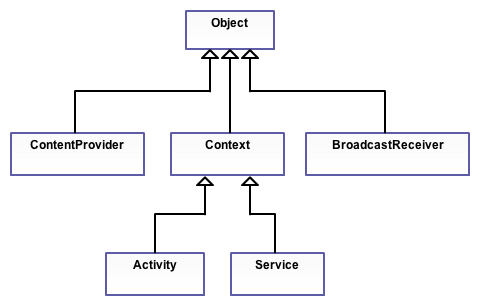
\includegraphics[width=130mm]{class_diagram.png}
\caption{Androidin tärkeimpien komponenttien luokkahierarkia} \label{class_diagram}
\end{figure}

Android-sovellukset koostuvat neljästä komponenttityypistä: aktiviteeteista (activities), palveluista (services), sisällöntarjoajista (content providers) sekä lähetysten vastaanottajista (broadcast receivers). Komponenttien välinen kommunikointi on pääosin tapahtumapohjaista; eri komponentit eivät keskustele suoraan keskenään, vaan kaikki siirtymät komponenttien välillä tapahtuvat käyttöjärjestelmän välittämien tapahtumaviestien perusteella. Tämän vaikutuksesta Android-sovellukset voivat helposti käyttää toiminnassaan järjestelmän ja toisten sovellusten tarjoamia komponentteja.

Kuvassa \ref{class_diagram} on esitelty Androidin peruskomponenttien muodostama luokkahierarkia. Vain aktiviteeteilla ja palveluilla on yhteinen yliluokka Context, lähetysten vastaanottajat ja sisällöntarjoajajat perivät vain Javan geneerisen Object-luokan. Kuvaa on yksinkertaistettu siten, että Contextin ja Activityn ja Servicen välillä olevia Wrapper-luokkia on jätetty kuvaamatta perintähierarkiassa. Context-luokka tarjoaa aktiviteettien ja palveluiden käyttöön sovelluksen globaaliin tilaan liittyviä tietoja.

Aktiviteetti kuvaa yhtä sovelluksen käyttöliittymän kerrallaan muodostavaa näkymää. Sovelluksen käyttöliittymä koostuu useista aktiviteeteista, jotka muodostavat yhtenäisen sovelluksen, mutta jokainen aktiviteetti on toisistaan riippumaton. Eri sovellukset voivat myös käynnistää toistensa aktiviteetteja, mikäli vastaanottava sovellus sen sallii. Esimerkiksi kamera-sovellus voi käynnistää sähköposti-sovelluksen sähköpostinkirjoitus-aktiviteetin, jos ottamansa kuvan haluaa jakaa sähköpostilla. Aktiviteetit ovat Androidissa Activity-luokan aliluokkia.

Palvelut ovat taustaprosesseja, jotka suorittavat pitkäkestoisia operaatioita, kuten tiedon lataamista verkosta tai musiikin soittamista taustalla samalla, kun käyttäjä käyttää toista sovellusta. Palvelut eivät tarjoa käyttöliittymää ja toiset komponentit, kuten aktiviteetit, voivat käynnistää niitä. Palvelut ovat Service-luokan aliluokkia.

Sisällöntarjoajat vastaavat sovelluksen tarvitseman tiedon lukemisesta ja kirjoittamisesta pitkäkestoiseen muistiin. Tallennuspaikkana voi olla laitteen tiedostojärjestelmä, SQLite-tietokanta, verkko tai ylipäänsä mikä tahansa kohde, johon sovelluksella on luku- tai kirjoitusoikeudet. Sovellukset voivat käyttää toistensa sisällöntarjoajia, mikäli sovellus julkaisee ne muiden sovellusten käyttöön. Sisällöntarjoajat ovat ContentProvider-luokan aliluokkia.

Lähetysten vastaanottajat reagoivat järjestelmänlaajuisiin viesteihin ja tapahtumiin. Tällaisia ovat esimerkiksi ilmoitus, että akku on lopussa tai että käyttäjä on sulkenut tai avannut näytön. Ne voivat myös lähettää järjestelmänlaajuisia tapahtumaviestejä muille sovelluksille. Lähetysten vastaanottajat ovat BroadcastReceiver-luokan aliluokkia, ja tapahtumat ovat Intent-luokan aliluokkia.

Android-sovellukset käyttävät usein hyväkseen toisten sovellusten komponentteja. Sovellukset eivät pysty suoraan kutsumaan toisiaan, vaan halutessaan hyödyntää toisten sovellusten ominaisuuksia sovellus luo uuden aikeen, jonka järjestelmä välittää tiettyjen sääntöjen perusteella sopivalle vastaanottajalle (katso luku \ref{intents}). 

Android-sovelluksilla ei ole yksittäistä main-metodia, joka käynnistäisi ohjelman, kuten usein muissa sovelluksissa on tapana. Sovellus voi sen sijaan käynnistyä vastaanottamansa aikeen johdosta monen eri komponentin kautta. Lisäksi sovellus saatetaan joutua käynnistämään ja sulkemaan useita kertoja esimerkiksi käyttäjän vaihtaessa puhelimen orientaatiota tai vastaanotettaessa puhelua, joten sovelluksen pitää pystyä tehokkaasti palautumaan keskeytyneeseen tilaansa. Sovelluksella on siis lukuisia mahdollisia käynnistymis- ja sulkeutumispolkuja. Tämän takia ohjelmakomponenttien elinkaaren hallinta on tärkeä osa sovelluksen rakentamista.

Android-sovelluksilla on xml-muotoinen Manifest-tiedosto, jossa määritellään sovelluksen komponentit, niiden näkyvyys ja minkälaisia tapahtumia ne osaavat hallita. Manifestissa määritellään myös mitä rajoitteita sovellus asettaa käytettävissä olevalle Android-versiolle, puhelimen ominaisuuksille, kuten lisälaitteiden saatavuudelle ja näyttöresoluutiolle, ja mitä oikeuksia sovellus vaatii toimiakseen. Näin voidaan varmistaa, että sovellusta ei asenneta laitteelle, jossa ei ole sovelluksen välttämättä tarvitsemia ominaisuuksia \cite{android}.

\subsection{Aktiviteetit}

\begin{figure}[htb]
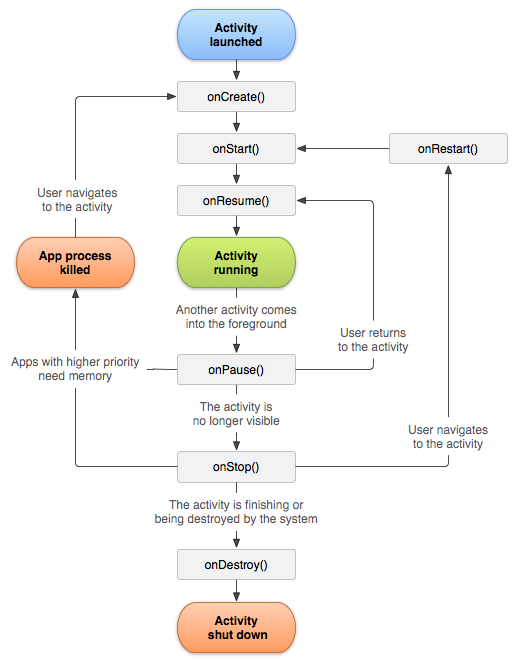
\includegraphics[width=100mm]{activity_lifecycle.png}
\caption{Aktiviteetin elinkaari} \label{activity_lifecycle}
\end{figure}

Aktiviteetti kuvaa yhtä sovelluksen käyttöliittymän näkymää. Lähes aina aktiviteetti on koko näytön kokoinen - eli kaikki, mitä puhelimen ruudulla näkyy yläreunan status-palkkia lukuunottamatta on samaa aktiviteettia - mutta ne voivat olla myös pienempiä tai leijua osittain toisen aktiviteetin päällä. Kuitenkin vain yksi aktiviteetti voi olla aktiivinen, eli reagoida käyttäjän syötteisiin, kerrallaan. Yksi sovelluksen aktiviteeteistä on yleensä pääaktiviteetti, joka käynnistyy silloin, kun käyttäjä avaa sovelluksen. 

Aktiviteettien elinkaaren hallinta on Android-sovelluksen kriittisimpiä osia, koska järjestelmän resurssit ovat yleensä hyvin rajalliset ja Android-laitteiden käyttöön liittyy usein tiheä vaihtelu eri sovellusten välillä. Tällöin on tärkeää, että sovellus luovuttaa varaamansa resurssit muiden sovellusten käyttöön, kun sovellus vaihtuu, ja vastaavasti osaa palautua takaisin pysäytettäessä olleeseen tilaan käyttäjän palatessa sovellukseen. Nämä vaihdokset pitäisi lisäksi tapahtua mahdollisimman tehokkaasti, jotta järjestelmän toiminta olisi käyttäjän näkökulmasta mahdollisimman sulavaa sovellusten tilojen vaihtamisen yhteydessä.

Aktiviteetilla voi olla pitkäkestoisemmin kolme eri tilaa. Aktiviteetti on aktiivisessa tilassa (resumed) silloin, kun se on näytön etualalla ja käyttäjä käyttää juuri sitä aktiviteettia. Keskeytetyssä (paused) tilassa aktiviteetti on, kun se on osittain näkyvissä, mutta jokin toinen aktiviteetti on aktiivisena sen päällä. Keskeytetyt aktiviteetit ja niiden tilat pysyvät muistissa, joskin jos laitteen muisti on lopussa, järjestelmä saattaa tuhota sen. Aktiviteetti on pysäytetty (stopped) silloin, kun jokin toinen aktiviteetti peittää sen kokonaan näkyvistä. Tällainenkin aktiviteetti säilyy muistissa, jos laitteen resurssit ovat riittävät, mutta järjestelmä voi tuhota sen koska vain, jos resursseja tarvitaan muiden aktiviteettien käyttöön.

Aktiviteetin siirtyminen eri tilojen välillä tapahtuu järjestelmän kutsuessa aktiviteetin takaisinkutsumetodeita. Mahdolliset tilasiirtymäpolut näkyvät kuvassa \ref{activity_lifecycle}. 

Aktiviteetin koko elinkaari tapahtuu onCreate()- ja onDestroy()-kutsujen välillä. Aktiviteetin tulisi tehdä kaikki kerran suoritettavat tilanalustustehtävät kutsuttaessa onCreate()-metodia, kuten ulkoasun määrittely tai koko aktiviteetin elinkaaren ajan tarvittavan tiedonsiirtosäikeen avaus. Vastaavasti onDestroy()-kutsussa aktiviteetin tulisi vapauttaa kaikki loputkin aktiviteetin varaamat resurssit.

Aktiviteetin käyttäjälle näkyvä elinkaari on onStart()- ja onStop()-kutsujen välillä. onStart()-metodia kutsutaan, kun aktiviteetti tulee näkyväksi käyttäjälle, ja onStop()-metodia kutsutaan, kun jokin toinen aktiviteetti on peittänyt kyseisen aktiviteetin kokonaan. Näkyvän elinkaaren aikana tulisi ylläpitää niitä resursseja, joita tarvitaan käyttäjän kanssa kommunikointiin sekä sellaisia, jotka saattavat muuten vaikuttaa käyttäjälle näkyvään käytöliittymään. Esimerkiksi lähetystenvastaanottajaa on hyvä kuunnella tällä välillä mahdollisten järjestelmänlaajuisten käyttöliittymään vaikuttavien tapahtumien varalta. onStart() ja onStop() -kutsuja voi tulla lukuisia aktiviteetin koko elinkaaren aikana. onRestart()-metodia kutsutaan, jos aktiviteetti on jo luotu aiemmin ja pysäytetty sitten onStop()-kutsulla. onRestart()-kutsua seuraa aina onStart()-kutsu.

Aktiviteetti on aktiivisena näytön etualalla onResume() ja onPause() -kutsujen välillä. Kun aktiviteetti on etualalla, käyttäjä käyttää juuri sitä ja se on kaikkien muiden aktiviteettien päällä. onResume() ja onPause() -kutsuja voi tulla tiheästi, esimerkiksi aina kun laitteen näyttö menee lepotilaan tai tulee jokin ilmoitus aktiviteetin päälle, joten niiden toteutus ei saa olla liian raskas.

Androidin järjestelmä voi tuhota sovelluksen prosessin onPausen(), onStopin() tai onDestroyn() jälkeen. Tämän takia pysyväksi tarkoitettu tieto on tallennettava onPause()-kutsun jälkeen. Tallennus voidaan tehdä esimerkiksi toteuttamalla takaisinkutsumetodi onSaveInstanceData(), jota kutsutaan aina, ennen kuin järjestelmä mahdollistaa aktiviteetin tuhoamisen. onSaveInstanceData() saa parametrinaan Bundle-olion, johon voi tallentaa tietoja nimi-arvo-pareina. Sama Bundle-olio tulee aktiviteetille onCreate() ja onRestoreInstanceState() -metodeille. Tiedon palautuksen voi tehdä kummassa tahansa näistä metodeista. Activity-luokka tarjoaa myös oletustoteutuksen onSaveInstanceData() ja onRestoreInstanceState()-metodeista, jotka osaavat monissa tapauksissa suorittaa tiedon tallennuksen ja palautuksen. Aktiviteetin tilanpalautusta tarvitaan usein, esimerkiksi aina kun käyttäjä vaihtaa sovelluksen suuntaa pysty- ja vaakasuuntien välillä.

Aktiviteettien vaihtumisen yhteydessä takaisinkutsujen järjestys on aina sama. Kun aktiviteetti A käynnistää aktiviteetti B:n, ensin kutsutaan aktiviteetti A:n onPause()-metodia, sitten aktiviteetti B:n onCreate(), onStart() ja onResume()-metodeita peräkkäin. Viimeiseksi kutsutaan aktiviteetti A:n onStop()-metodia, mikäli aktiviteetti B peittää sen kokonaan. Näin esimerkiksi aktiviteetti A:n onPause()-metodissa tietokantaan tallennetut tiedot ovat käytössä aktiviteetti B:tä käynnistettäessä. Jos muutoksia taas tekee onStop()-metodissa, ne tapahtuvat vasta aktiviteetti B:n käynnistyttyä.

\subsubsection*{Palat}

Androidin versiosta 3 (API-versio 11) asti on ollut mahdollista määritellä aktiviteetteihin paloja (Fragment-luokan aliluokkia). Palat ovat uudelleenkäytettäviä komponentteja, joita voi käyttää osana aktiviteetteja. Niiden avulla on helpompi luoda käyttöliittymiä, jotka skaalautuvat eri kokoisille näytöille. Isommalla näytöllä aktiviteetti voi pitää sisällään useita paloja, jotka pienemmällä näytöllä ovatkin omissa aktiviteeteissaan. Palojen elinkaari on riippuvainen siitä aktiviteetista, johon ne on sisällytetty. Kun aktiviteetti pysähtyy, niin pysähtyy myös aktiviteetin sisältämät palat. Samoin aktiviteetin tuhoutuessa tuhoutuvat myös palat. Aktiviteettien sisällä paloilla voi kuitenkin olla oma elinkaarensa, niitä voi käynnistää ja tuhota vapaasti aktiviteetin ollessa käynnissä.

Palojen elinkaarta hallitaan takaisinkutsumetodeilla, kuten aktiviteettejakin. Monet metoditkin ovat samoja, kuten onCreate(), onStart(), onPause() ja onStop(). Lisäksi paloilla on muutamia takaisinkutsumetoideita, joita aktiviteeteilla ei ole. onCreateView()-metodia kutsutaan, kun palan käyttöliittymä tulee ensimmäistä kertaa näkyviin käyttäjälle. onAttach()-metodia kutsutaan, kun pala on liitetty johonkin aktiviteettiin. Tällöin pala saa itselleen viitteen aktiviteettiin kommunikointia varten. onActivityCreated()-metodia kutsutaan, kun palan liittäneen aktiviteetin onCreated()-metodi on ajettu. onDestroyView()-metodia kutsutaan, kun palan käyttöliittymä tuhotaan, ja onDetach()-metodia kutsutaan kun palaan liitetty aktiviteetti irroitetaan palasta \cite{android}.

\subsection{Palvelut}

\begin{figure}[htb]
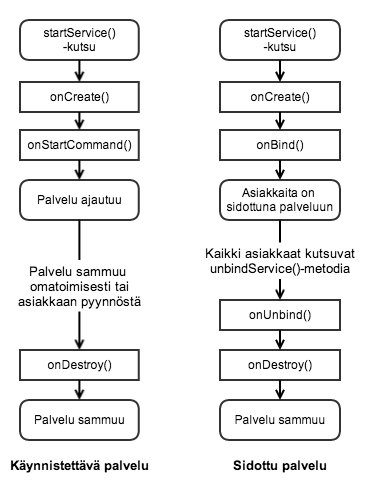
\includegraphics[width=100mm]{service_lifecycle.png}
\caption{Palvelun elinkaari} \label{service_lifecycle}
\end{figure}

Palvelut ovat pitkäkestoisia taustaoperaatioita. Muut sovelluskomponentit voivat käynnistää niitä, ja ne jatkuvat vaikka käyttäjä lopettaisi kyseisen sovelluksen käyttämisen. Palvelu voi esimerkiksi soittaa musiikkia, suorittaa verkkotransaktioita, kommunikoida sisällöntarjoajien kanssa tai tehdä levykirjoitusta.

Palvelut voivat olla kahdenlaisia. Käynnistettävät (\emph{started}) palvelut suorittavat tehtävänsä kun niiden startService()-metodia kutsutaan. Tällainen palvelu voi jatkaa pyörimistä taustalla, vaikka sovellus suljettaisiin. Tyypillisesti käynnistettävä palvelu tekee jonkin yhden operaation, kuten tiedoston latauksen tai lähettämisen, ja lopettaa sitten itsensä. Käynnistettävät palvelut eivät yleensä palauta palautusarvona kutsujalle mitään. Käynnistettävien palveluiden tulee sulkea itsensä operaation valmistuttua kutsumalla stopSelf()-metodia. Myös muut komponentit voivat sulkea palvelun kutsumalla stopService()-metodia.

Sidotut (\emph{bound}) palvelut ovat sellaisia, että sovelluskomponentit sitovat palvelun niihin kutsumalla bindService()-metoida. Sidotut palvelut tarjoavat asiakas-palvelin-rajapinnan sitovalle komponentille. Palvelu voi vastaanottaa pyyntöjä ja palauttaa vastauksia niihin. Palvelun elinkaari on sama kuin sen sitoneen komponentin. Useampi komponentti voi sitoa saman palvelun yhtä aikaa. Tällöin palvelu sulkeutuu kun viimeinenkin niistä lopettaa toimintansa. Sitominen vapautetaan kutsumalla unbindService()-metodia.

Useimmiten käynnistettävät ja sidotut palvelut ovat erillisiä, mutta joissain tilanteissa sama palvelu voi toimia sekä käynnistettävänä että sidottuna palveluna. Käynnistettäviä palveluita käytetään tyypillisesti pitkäkestoisiin taustaoperaatioihin, jotka suoritetaan taustalla ilman että käyttäjä puuttuu niiden toimintaan. Sidotut palvelut taas voivat tarjota sovellukselle minkä tahansa palvelurajapinnan, jonka kanssa sovellus voi kommunikoida palvelun elinkaaren ajan.

Palveluiden elinkaari on esitetty kuvassa \ref{service_lifecycle}. Aktiviteettien tavoin koko palvelun elinkaari tapahtuu onCreate() ja onDestroy()-kutsujen välissä ja palvelun alustus tapahtuu onCreate()-metodissa. Sidotun palvelun aktiivinen elinkaari on onBind() ja onUnbind()-kutsujen välillä. Käynnistettävän palvelun elinkaari puolestaan alkaa onStartCommand()-kutsusta kunnes se sulkee itsensä stopSelf()-kutsulla. onBind() ja onStartCommand() -metodit saavat parametrinaan aikeen, jonka niitä kutsunut komponentti antoi bindService() tai startService() -metodille \cite{android}.

\subsection{Sisällöntarjoajat}

Sisällöntarjoajat tarjoavat pääsyn pysyvästi tallennettuun tietoon. Ne kapsuloivat tiedon ja tarjoavat mekanismit tiedon yksityisyyden hallintaan. Sisällöntarjoajat toimivat rajapintana tiedon ja sovelluskoodin välillä. Kun sisällöntarjoajan tietoon halutaan päästä käsiksi, käytetään ContentResolver-oliota Context-luokassa, joka sitten kommunikoi itse sisällöntarjoajan kanssa.

Sisällöntarjoajat eivät ole välttämättömiä sovelluksessa, jos tietoon ei haluta päästä käsiksi muista kuin samasta sovelluksesta. Sovellustenväliseen kommunikointiin sisällöntarjoajat tarjoavat vakiorajapinnan, joka pitää huolen prosessienvälisestä kommunikoinnista ja tietoturvallisuudesta.

Androidin mukana tulee valmiiksi toteutetut sisällöntarjoajat esimerkiksi musiikille, videotiedostoille ja käyttäjän yhteystiedoille. Muutamia rajoitteita lukuunottamatta nämä sisällöntarjoajat ovat kaikkien sovellusten käytettävissä \cite{android}.

\section{Aikeet}
\label{intents}

Suurin osa Android-sovellusten kommunikaatiosta on tapahtumapohjaista. Niin aktiviteetit, palvelut kuin sisällöntarjoajatkin käynnistetään lähettämällä niille aie (\emph{intent}). Tapahtumia käytetään Androidissa, koska niiden avulla komponentit voidaan sitoa toisiinsa ajonaikaisesti ja vasta silloin, kun niitä varsinaisesti tarvitaan. Itse aie-oliot ovat passiivisia tietorakenteita, joissa on abstrakti kuvaus operaatiosta, joka halutaan suoritettavan, tai lähetysten (\emph{broadcast}) tapauksessa kuvaus siitä, mitä on tapahtunut. 

Aikeiden kohde voidaan nimetä ekspliittisesti ComponentName-kentässä. Tällöin annetaan kohdekomponentin täydellinen nimi paketteineen, jolloin kohde voidaan tunnistaa yksikäsitteisesti. Tämän muodon käyttäminen vaatii, että kutsuva komponentti tietää kohdekomponentin nimen. Sovelluksensisäisessä kommunikoinnissa tämä onnistuu, mutta sovellustenvälisessä kommunikoinnissa useinkaan ei. Tällöin kohde päätellään implisiittisesti muista aikeelle annetuista kentistä.

Action-kentässä annetaan tapahtuma, joka aikeella halutaan käynnistää, esimerkiksi puhelun aloitus, tai lähetysten vastaanottajien tapauksessa järjestelmässä tapahtunut tapahtuma, kuten varoitus akun loppumisesta. Intent-luokassa määritellään lukuisia vakioita erilaisia tapahtumia varten, mutta niiden lisäksi sovellukset voivat määritellä myös omia tapahtumia.

Data-kentässä annetaan tapahtumaan liittyvän tiedon osoite (URI) ja tyyppi (MIME). Näin vastaanottava komponentti tietää minkätyyppistä tietoa aikeeseen liittyy, ja mistä se löytyy. Category-kentässä kerrotaan, minkä tyyppisen komponentin odotetaan käsittelevän aikeen. Näitäkin Intent-luokka tarjoaa valmiita, mutta omien käyttö on mahdollista.

Aikeen vastaanottava komponentti voidaan päätellä kahdella tavalla. Komponentti valitaan ekplisiittisesti, jos ComponentName-kentässä on arvo. Tällöin muiden kenttien arvoista ei välitetä. Muussa tapauksessa Action-, Data- ja Category-kenttien arvojen perusteella selvitetään, mitä soveltuvia vastaanottavia komponentteja järjestelmään on asennettuna. Tässä käytetään apuna aiesuotimia (Intent filter).

Sovellukset voivat määritellä aiesuotimia, jotta järjestelmä tietää, mitkä sovellukset voivat ottaa vastaan aikeita. Aiesuotimet ovat komponenttikohtaisia, ja ne määrittelevät, mitä tapahtumia, tietotyyppejä ja kategorioita ne tukevat. Aiesuotimia käytetään hyväksi implisiittisessä kohteen määrittelyssä. Jos kohde on määritelty eksplisiittisesti komponentin nimellä, aiesuotimilla ei ole vaikutusta \cite{android}.

\subsection{Android manifest}

Jokaisella Android-sovelluksella on AndroidManifest.xml-tiedosto, joka sisältää järjestelmälle välttämätöntä tietoa sovelluksen ajamiseksi. Manifestissa määritellään muunmuassa sovelluksen javapaketti, joka toimii samalla sovelluksen uniikkina tunnisteen, määritellään sovelluksen komponentit, eli aktiviteetit, palvelut, sisällöntarjoajat ja lähetysten vastaanottajat, joista sovellus koostuu, sekä niiden toiminnallisuus ulkopuolelta tulevien aikeiden kannalta, mitä oikeuksia sovellus tarvitsee toimiakseen, mitä oikeuksia toisilla sovelluksilla pitää olla, jotta ne voivat käyttää kyseisen sovelluksen palveluita, mikä on sovelluksen vaatima Android API:n minimiversio sekä mitä kirjastoja sovellus tarvitsee toimiakseen. \cite{android}
\clearpage
\section{Testaamisesta, testityökalujen arvioinnista ja mobiilisovellusten testaamisen erityispiirteistä}

Jotain

\subsection{Testaamisen peruskäsitteitä}

Testitapaus (test case) on yksittäinen testi, jolle on määritelty syötteet, suoritusehdot ja läpäisykriteerit. Testisarja (test suite) taas on joukko testitapauksia. Testisarja voi myös koostua useasta testisarjasta, jolloin esimerkiksi ohjelman jokaiselle komponentille voi olla oma testisarjansa ja yksi testisarja kattaa sitten kaikki yksittäisten komponenttien testisarjat. \cite[153]{testing}

Yksikkötestauksella (unit testing) tarkoitetaan testejä, joiden kohteena on pienimmät mahdolliset ohjelmakomponentit. Olio-ohjelmoinnissa tämä tarkoittaa useimmiten yksittäistä luokkaa, koska yksittäiset metodit vaikuttavat olion tilaan ja siten metodien toimintaan. \cite[282-286]{testing}. JUnit \cite{junit} on Javan standardi yksikkötestaustyökalu.

Yksikkötestaus on useimmiten valkoinen laatikko -testausta (white box testing / structural testing / glass box testing), jolloin testejä voidaan kirjoittaa ohjelmakoodin perusteella. Testeiltä voidaan vaatia esimerkiksi tiettyä koodikattavuutta, jolloin varmistetaan, että mahdollisimman suuri osa ohjelmakoodista tulee suoritettua testien aikana. \cite[154]{testing}

Toiminnallisessa testauksessa (functional testing) testattavan ohjelman sisäistä rakennetta ei tunneta vaan ollaan kiinnostuttu vain syötteistä ja niitä vastaavista tulosteista. Toiminnallista testausta voidaan kutsua myös musta laatikko -testaukseksi (black box testing) (varmista jostain toisesta lähteestä että nämä ovat oikeasti synonyymi, wikipedian mukaan ei ole vaan functional on black boxin alalaji!) Toiminnallisessa testauksessa ollaan kiinnostuttu ohjelman käyttäjälle näkyvästä toiminnasta ja niitä voidaan tehdä esimerkiksi ohjelman määrittelyn pohjalta. \cite[161-162]{testing}

Mallipohjainen testaus (model based testing) on toiminnallisen testauksen alalaji, jossa testitapaukset luodaan automaattisesti ohjelman spesifikaatiosta tehdystä mallista. Jos ohjelma mallinnetaan formaalilla mallilla, kuten äärellisellä automaatilla tai kieliopilla, voidaan testitapaukset generoida täysin automaattisesti. Semiformaaleilla menetelmillä, kuten luokka- tai oliokaavioilla, mallinnetuista ohjelmista generointi saattaa vaatia manuaalista työtä. \cite[245-250]{testing}

Järjestelmätestauksessa (system testing) testataan koko järjestelmää, se perustuu ohjelman havaittavaan toimintaan ja se on itsenäinen suhteessa ohjelman toteutukseen. Jos ohjelma läpäisee järjestelmätestit, sen voi olettaa olevan vapaa tunnetuista bugeista. \cite[418-421]{testing}

Hyväksyntätestien (acceptance tests) tarkoitus on kertoa, onko ohjelma valmist julkaistavaksi. Hyväksyntätesteissä ei etsitä vikoja ohjelmasta, vaan yritetään varmistaa sen riittävä laatutaso. Hyväksyntätestit ovat usein tilastollisia: niissä mitataan ohjelman luotettavuutta, saavutettavuutta tai häiriötiheyttä. Ongelmana tällaisessa testauksessa on, että vaatii hyvin paljon testiainestoa ennen kuin voidaan olla varmoja ohjelman riittävästä laadusta. Usein hyväksyntätestauksessa käytetään alfa- ja beta-testausta, jolloin ohjelman käyttäjät pääsevät testaamaan ohjelmaa ja raportoimaan sen laadusta. \cite[421-423]{testing}

Mockaus (suomennos?) on tekniikka, joka helpottaa yksikkötestien kirjoittamista. Yksikkötestien ulkoiset riippuvuudet voidaan korvata testeissä kontrolloitavilla mock-olioilla. Tällöin testit ovat vakaampia, koska ulkopuolisten komponenttien muokkaus ei vaikuta testeihin, testin haluttuun lopputulokseen vaikuttava ympäristö on helppo saada haluttuun muotoon. Tällöin testien on helppo testata myös sellaisia olosuhteita, jotka ovat harvinaisia, tai vaikea saada muokattua. Lisäksi mockaamalla voidaan korvata vielä tekemättömät ulkoiset riippuvuudet mock-toteutuksilla. \cite{mocking}

\subsection{Mikä on hyvä testityökalu?}

Androidille on tehty Androidin mukana tulevien testaustyökalujen lisäksi monia muita testaustyökaluja. Nämä työkalut erottautuvat Androidin työkaluista jollain tavalla.

Testaustyökalujen arviointia käsittelevät muunmuassa Poston ja Sexton \cite{poston92}. Hyvän testaustyökalun kriteerit ovat osin kontekstista riippuvia, mutta Poston ja Sexton määrittelevät myös yleisempiä kriteerejä testityökalujen arviointiin. Työkalun toiminnallisten ominaisuuksien arviointi on yleensä kontekstiriippuvaista, mutta usein myös helposti määriteltävissä. Jollain työkalulla pystyy testaamaan asioita, joita toisella ei voi. Ei-toiminnallisia olennaisia ominaisuuksia he luettelevat työkalun tehokkuuden, miten nopeasti sen käytön oppii, miten nopeaa testien tekeminen sillä on ja miten luotettava työkalu on.
\clearpage
\section{Android-sovellusten testaaminen ja Androidin mukana tulevat testityökalut}

Androidin sovelluskehityspaketin mukana tulee monia Googlen kehittämiä testaustyökaluja. Esittelen niitä tässä luvussa. Samalla tutustutaan Android-sovelluksen testaamisen perusteisiin.

\subsection{Android-testien ajoympäristö}

\begin{figure}[htb]
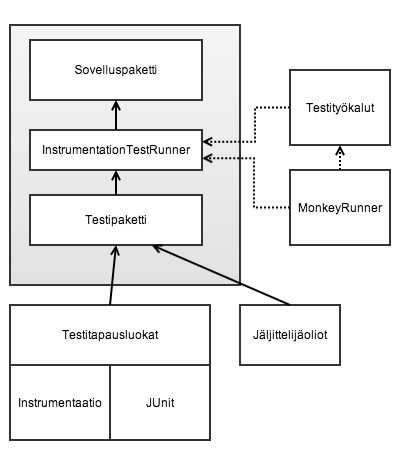
\includegraphics[width=100mm]{test_framework.png}
\caption{Android-testien ajoympäristö} \label{test_framework}
\end{figure}

Androidin-sovelluksen testejä voi ajaa joko emulaattorilla tai suoraan puhelimessa. Androidin testisarjat perustuvat JUnit-testikehikkoon. Puhdasta JUnitia voi käyttää sellaisen koodin testaamiseen, joka ei kutsu Androidin rajapintaa tai sitten voi käyttää Androidin JUnit-laajennusta Android-komponenttien testaukseen. Laajennus tarjoaa komponenttikohtaiset yliluokat testitapausten kirjoittamista varten. Nämä luokat tarjoavat apumetodeita jäljittelijöiden (mock object) luomiseen ja komponentin elinkaaren hallintaan. Androidin JUnit-toteutus mahdollistaa JUnitin versio 3:n mukaisen testityylin, ei uudempaa versio 4:n mukaista.

Kuvassa \ref{test_framework} on esitetty Androidin testien ajoympäristö. Testattavaa sovellusta testataan ajamalla testipaketissa olevat testitapaukset MonkeyRunnerilla (ks. luku \ref{monkeyrunner}). Testipaketti sisältää testitapausten lisäksi Androidin instrumentaatiota, eli apuvälineitä sovelluksen elinkaaren hallintaan ja koukkuja, joilla järjestelmän lähettämiä callback-metodikutsuja pääsee muokkaamaan, sekä jäljittelijäolioita korvaamaan järjestelmän oikeita luokkia testin ajaksi jäljittely-toteutuksella. \cite{android}

\subsection{Komponenttikohtaiset yksikkötestiluokat}

Android tarjoaa aktiviteeteille, palveluille ja sisällöntarjoajille jokaiselle oman testiyliluokkansa, joka mahdollistaa komponenttikohtaisten testien helpomman toteutuksen.

Aktiviteettien testauksessa Androidin JUnit-laajennus on merkittävä, koska aktiviteeteilla on monimutkainen elinkaari, joka perustuu paljolti takaisinkutsumetodeihin, joiden suora kutsuminen ei ole mahdollista. Aktiviteettien testauksen pääyliluokka on InstrumentationTestCase. Sen avulla on mahdollista käynnistää, pysäyttää ja tuhota testattavana oleva aktiviteetti halutuissa kohdissa. Lisäksi sen avulla voi jäljitellä järjestelmäolioita, kuten Context- ja Applications-luokan instansseja. Tämä mahdollistaa testin eristämisen muusta järjestelmästä ja aikeiden luomisen testejä varten. Lisäksi yliluokassa on metodit käyttäjän vuorovaikutusten, kuten kosketus- ja näppäimistötapahtumien lähettämiseen suoraan testattavalle luokalle.

Aktiviteettien testaamiseen on kaksi välitöntä yliluokkaa, ActivityUnitTestCase ja ActivityInstrumentationTestCase2. ActivityUnitTestCase on tarkoitettu luokan yksikkötestaamiseen siten, että se on eristetty Android-kirjastoista. Näitä testejä voi ajaa suoraan kehitystyökalu ja tarvittaessa Android-kirjaston mockaamiseen on käytössä MockApplication-olio. ActivityInstrumentationTestCase2 taas on tarkoitettu toiminnalliseen testaukseen tai useamman aktiviteetin testaamiseen. Ne ajetaan normaalissa suoritusympäristössä emulaattorilla tai Android-laitteessa. Aikeiden jäljittely on mahdollista, mutta testin eristäminen muusta järjestelmästä ei ole mahdollista.

Palveluiden testaaminen on paljon yksinkertaisempaa kuin aktiviteettien. Ne toimivat eristyksessä muusta järjestelmästä, joten testattaessakaan ei tarvita Androidin instrumentaatiota. Android tarjoaa ServiceTestCase-yliluokan palveluiden testaamiseen. Se tarjoaa jäljittelijäoliot Application- ja Context-luokille, joten palvelun saa testattua eristettynä muusta järjestelmästä. Testiluokka käynnistää testattavan palvelun vasta kutsuttaessa sen startService() tai bindService()-metodia, jolloin jäljittelijäoliot voi alustaa ennen palvelun käynnistymistä. Jäljittelijäolioiden käyttö palveluiden testaamisessa paljastaa myös mahdolliset huomaamatta jääneet riippuvuudet muuhun järjestelmään, koska Jäljittelijäoliot heittävät poikkeuksen, mikäli niihin tulee metodikutsu, johon ei ole varauduttu.

Sisällöntarjoajien testaaminen on erityisen tärkeää, jos sovellus tarjoaa sisällöntarjoajiaan muiden sovellusten käyttöön. Tällöin on myös olennaista testata niitä käyttäen samaa julkista rajapintaa, jota muut sovellukset joutuvat käyttämään kommunikoidessaan sisällöntarjoajien kanssa. Sisällöntarjoajien testauksen yliluokka on ProviderTestCase2, joka tarjoaa käyttöön jäljittelijäoliot ContentResolveriosta ja Contextista, jolloin sisällöntarjoajia voi testaja eristyksissä muusta sovelluksesta. Yliluokka tarjoaa myös metodit sovelluksen oikeuksien testaamisen. Contextin jäljittelijäolio mahdollistaa tiedosto- ja tietokantaoperaatiot, mutta muut Androidin kirjastokutsut on toteutettu tynkinä (stub). Lisäksi tiedon kirjoitusosoite on uniikki testissä, joten testien ajaminen ei yliaja varsinaista sovelluksen tallentamaa tietoa. Sisällöntarjoajatestit ajetaan emulaattorissa tai Android-laitteella. \cite{android}

\subsection{MonkeyRunner}
\label{monkeyrunner}

MonkeyRunner tarjoaa rajapinnan, jolla Android-sovellusta voi ohjata laitteessa tai emulaattorissa. Se on lähinnä tarkoitettu toiminnallisten testien sekä yksikkötestien ajamiseen, mutta soveltuu myös muihin tarkoituksiin. Sen avulla voi esimerkiksi asentaa sovelluksia, ajaa testisarjoja ja sovelluksia ja lähettää niihin syötteitä. Lisäksi monkeyrunnerilla voi ottaa eri kohdista kuvakaappauksia ja verrata niitä referenssikuviin. Tällä tavalla voidaan tehdä esimerkiksi regressiotestausta.

MonkeyRunnerilla voidaan testata yhtä aikaa monia eri emulaattoreita tai useita laitteita, jolloin voidaan tehdä fragmentaatiotestausta. MonkeyRunner on myös laajennettavissa, jolloin sitä voi käyttää muihinkin tarkoituksiin. MonkeyRunneria ohjataan pythonilla ja se on toteutettu jythonilla, joka on Javan virtuaalikoneessa pyörivä python-toteutus \cite{android}.

\subsection{Uiautomator ja Uiautomatorviewer}

Uiautomator tarjoaa mahdollisuuden kirjoittaa toiminnallisia mustalaatikko-testejä Android-sovelluksille Monkeyrunneria paremmat assert-mahdollisuudet ja mahdollisuuden toiminallisten musta laatikko -testien kirjoittamiseen Javalla tarjoaa Uiautomator. Siinä on kaksi komponenttia: Uiautomatorviewer ja Uiautomator. Uiautomatorviewer on graafinen työkalu, jolla voi analysoida ja skannata Android-sovelluksen käyttöliittymää ja Yiautomator työkalu, joka tarjoaa rajapinnan ja moottorin toiminnallisten mustalaatikkotestien ajamiseen.

\begin{figure}[htb]
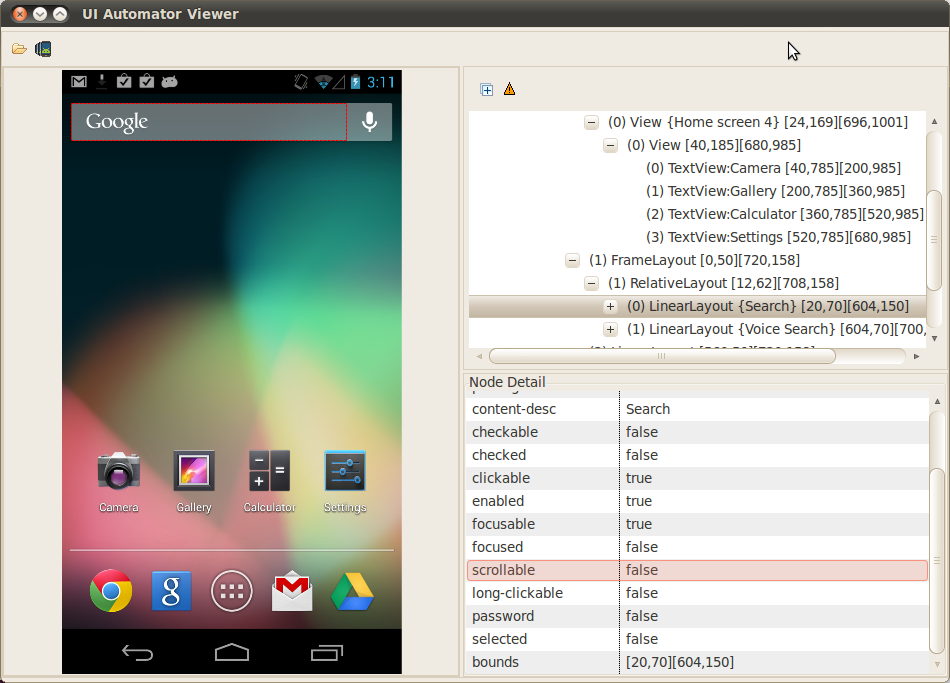
\includegraphics[width=160mm]{uiautomatorviewer.png}
\caption{UIAutomatorViewerin käyttöliittymä} \label{uiautomatorviewer}
\end{figure}

Uiautomatorviewer (kuvassa \ref{uiautomatorviewer}) analysoi sovelluksen näkymän komponentit. Vasemmalla näkymässä punaisella ympyröitynä on oikeasta valikosta valittu komponentti. Oikeassa alareunassa näytetään komponentin tietoja, joita voi käyttää testeissä esimerkiksi komponentin valitsijoissa, esimerkiksi siten, että valitaan save-nappi tekstin perusteella, jotta siitä voidaan testissä painaa.

Uiautomator-testit kirjoitetaan Javalla JUnitiin pohjautuen perimällä UIAutomatorTestCase-yliluokka, joka tarjoaa käyttöön käyttöliittymäelementtien valitsemiseen tarvittavan rajapinnan ja mahdollisuuden vuorovaikutukseen niiden kanssa. UISelector-luokassa on metodeita käyttöliittymäelementtien valitsemiseen ja UIObject-luokassa niiden kanssa kommunikointia varten. UIObject-oliolta voi kysyä assertointia varten elementin olemassaoloa ja erilaisia tilaan liittyviä tietoja, kuten onko elementti käytössä tai painettavissa.

Uiautomator on uusi työkalu ja testejä voi ajaa vain laitteilla, jotka tukevat API:n versiota 16 tai uudempaa. Tämä vastaa Androidin versiota 4.1, joka on julkaistu kesäkuussa 2012. Uiautomatorilla ei voi siis testata sovellusta vanhemmilla Android-laitteilla, joita on tällä hetkellä vielä reilusti yli puolet Androidin laitekannasta \cite{android}.

\subsection{Monkey}

Monkey on Androidin mukana tuleva työkalu, jota voi ajaa emulaattorissa tai Android-laitteessa ja joka tuottaa sovellukselle pseudosatunnaisia syötteitä. Näitä voi olla esimerkiksi painallukset, eleet sekä järjestelmätason viestit. Monkeytä voi käyttää esimerkiksi sovelluksen stressitestaukseen tai fuzz-testaukseen.

Monkeylle voi antaa jonkin verran sen toimintaa ohjaavia parametreja. Ensinnäkin testisyötteiden määrää ja tiheyttä voi rajoittaa. Toiseksi erityyppisten syötteiden osuutta voi säätää. Kolmanneksi testauksen voi rajoittaa tiettyyn pakettiin sovelluksessa. Tällöin Monkey pysäyttää testauksen, jos se on ajautuu muihin kuin haluttuun osaan sovelluksesta. Neljänneksi Monkeyn tulosteiden määrää ja tarkkuutta voi säätää.

Monkey pystäyttää testin, jos ohjelmasta lentää käsittelemätön poikkeus tai jos järjestelmä lähettää sovellus ei vastaa -virheviestin. Näissä tapauksissa Monkey antaa raportin virheestä ja miten se syntyi. Monkey voi myös tehdä profilointiraportin testistä.\cite{android}
\clearpage
\section{Yksikkötestityökalujen vertailua}

Androidin yksikkötestaustapa on tehdä JUnit-testejä Androidin oman AndroidUnitTestCase-luokan aliluokkana. Nämä testit ajetaan emulaattorissa Dalvik-ympäristössä. Tässä tavassa on kaksi heikkoutta, jonka takia on kehitetty myös kolmansien osapuolien yksikkötestityökaluja Android-ympäristöön. Ensinnäkin testien ajaminen emulaattorissa on hitaampaa, kuin jos niitä voisi ajaa suoraan tavallisessa Javan virtuaalikoneessa JUnit-testeinä. Toiseksi muutkaan testauksen apuna käytettävät työkalut, kuten jäljittelijä-työkalut, eivät välttämättä toimi ongelmitta Dalvik-ympäristössä. Tässä luvussa vertailen Android-sovelluksen yksikkötestausta AndroidUnitTestCasella ja suosituimmalla Javan virtuaalikoneessa pyörivällä vaihtoehdolla: Robolectricillä. Tavoitteena on selvittää, voiko Robolectricillä helposti korvata Androidin oman yksikkötestikehyksen ja pitääkö Robolectricin lupaus nopeammasta testien suoritusajasta paikkansa.

Android-sovellusten yksikkötestauksessa kiinnostavaa on nimenomaan Androidin kirjastoluokista perivien keskeisten komponenttien testaus, koska sovelluksessa mahdollisesti olevat muut kuin Androidin kirjastoluokista perivät luokat on helppo testata tavanomaisilla Javan yksikkötestityökaluilla ilman erityisesti Androidille tarkoitettuja työkaluja samaan tapaan kuin muutkin Java-sovellukset.

Yksikkötestaustyökaluissa tärkeintä on nopeus, jotta tdd-kehityssykli toimisi mahdollisimman nopeasti, työkalun käytön helppous ja koodin ytimekkyys, jotta testien kirjoittaminen sujuu nopeasti, sekä yhteensopivuus jäljittelijäkehysten kanssa, jotta komponenttien yksikkötestaus muusta sovelluksesta eristettynä olisi mahdollista.

\subsection{Robolectric}

Robolectric on yksikkötestaustyökalu, jonka tarkoitus on mahdollistaa Android-koodin yksikkötestaus suoraan ohjelmointiympäristössä Javan virtuaalikoneessa ilman emulaattoria. Tarkoitus on mahdollistaa nopea tdd-sykli ja helpompi integrointi jatkuvan integroinnin palveluihin. Normaalisti Android-kirjaston luokat palauttavat kutsuttaessa ohjelmointiympäristöstä ajoaikaisen poikkeuksen, mutta Robolectric korvaa nämä luokat varjototeutuksilla, jotka palauttavat poikkeuksen sijaan tyhjän oletusvastauksen, kuten null, 0 tai false, tai jos Robolectricissa on kyseistä metodia varten olemassa varjototeutus, se palauttaa toteutuksen määrittelemän paluuarvon.

Robolectricin varjoluokkien käytön vaihtoehtona on jonkin jäljittelijäkehyksen käyttäminen Androidin kirjaston korvaamiseen, mutta tämä tapa kirjoittaa testejä on hyvin työläs, koska koodirivejä kertyy väistämättä paljon. Lisäksi tällöin testejä kirjoitettaessa täytyy tuntea testattavan metodin toiminta hyvin tarkasti, jotta jäljittelijätoteutukset saadaan kirjoitettua. Robolectricin varjoluokat mahdollistavat enemmän musta laatikko -tyyppisen testauksen \cite{robolectric}.

\subsection{Aiempaa tutkimusta}

Sadeh et al. vertasivat Androidin aktiviteettien yksikkötestausta JUnitilla, Androidin omilla yksikkötestityökaluilla sekä Robolectricilla \cite{sadehetal11}. JUnitilla testattaessa ongelmaksi muodostui, että ohjelmakoodia jouduttiin melko rajusti muokkaamaan, jotta luokkien yksikkötestaus onnistui. Tämä tekee ohjelman ylläpidon vaikeaksi. JUnitin hyvä puoli oli erittäin nopea testien ajonopeus. Robolectricillä testien tekeminen taas oli lähes yhtä helppoa kuin Androidin omilla työkaluilla. Androidin työkaluihin verrattuna Robolectricin vahvuudet olivat virhepaikkojen paikantamisen helppous ja testien suoritusnopeus. Robolectric-testit ajautuivat viisi kertaa nopeammin kuin Androidin työkaluilla ajetut testit, koska Androidin työkaluilla kirjoitetut testit ajetaan Dalvik-emulaattorilla, Robolectric taas suoraan Javalla. Androidin omien työkalujen suurin vahvuus oli testien kirjoittamisen helppous.

Sadeh et al. eivät käyttäneet JUnit-testeissään mitään jäljittelijätyökalua, joten testeissä testiluokan riippuvuudet jäljiteltiin tekemällä niistä staattisia sisäluokkia testiluokan sisään. Tämä vaatii paljon koodia ja vaikutti osaltaan siihen, miksi puhdas JUnit-testi näytti niin hankalalta. Androidin kirjastoluokat on pakko eristää testattavasta luokasta Javan virtuaalikoneella testattaessa, koska Androidin kehitysympäristössä käytettävä paketti ei sisällä varsinaisesti luokkien sisältöä, vaan vain niiden luokkien julkiset rajapinnat, jolloin kehitystyökalut osaavat auttaa niiden käytössä, mutta varsinaista toteutusta ei ole.

Jeon \& Foster \cite{troyd} mainitsevat Robolectricin vahvuudeksi sen, että se pyörii Javan virtuaalikoneessa ja näin ohittaa testeistä hitaan vaiheen, jossa sovellus pitää kääntää emulaattorille tai laitteelle testattavaksi. Robolectric ei heidän mielestään kuitenkaan sovellu kokonaisten sovellusten testaamiseen, koska sen varjoluokat eivät toteuta Androidin komponenteista kuin osan.

Allevato \& Edwards \cite{robolift} käyttivät Robolectriciä opetuskäyttöön tarkoitetun RoboLIFT-työkalun kehitykseen. Robolectric auttoi heitä ohittamaan emulaattorin käytön ja nopeuttamaan opiskelijoiden testisykliä ja automaattista arviointialgoritmia. Tässä käytössä Robolectricin ongelma oli, että se ohittaa käyttöliittymän piirtämisen kokonaan ja muunmuassa näkymien onDraw()-metodia ei kutsuta ollenkaan. Tämän seurauksena esimerksi näkymän leveys on aina 0 pikseliä, jolloin sellaiset testit, joilla haluttiin klikata näytöllä johonkin suhteelliseen kohtaan (vaikkapa keskelle) eivät toimineet oikein.

\subsection{Testiprojekti}

\begin{figure}[h]
\centering
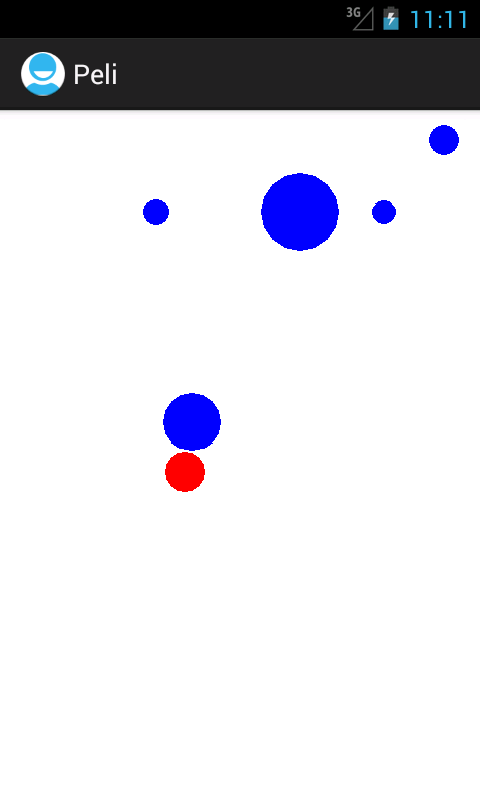
\includegraphics[width=60mm]{peli_screenshot.png}
\caption{Ruutukaappaus testiohjelman pelinäkymästä} \label{peli_screenshot}
\end{figure}

Yksikkötestaustyökaluja testasin itse tehdyllä demoprojektilla. Kyseessä on yksinkertainen peli, jonka pelinäkymästä on ruutukaappaus kuvassa \ref{peli_screenshot}. Pelissä ohjataan kosketusnäytöllä painamalla punaista palloa ja pyritään väistämään ympäriinsä pomppivia sinisiä palloja. Kun peli päättyy, palataan takaisin päänäkymään, josta on ruutukaappaus kuvassa \ref{mainactivity}. Tästä näkymästä voi aloittaa uuden pelin ja lisäksi näkee, montako sekuntia edellinen peli kesti.

\begin{figure}[h]
\centering
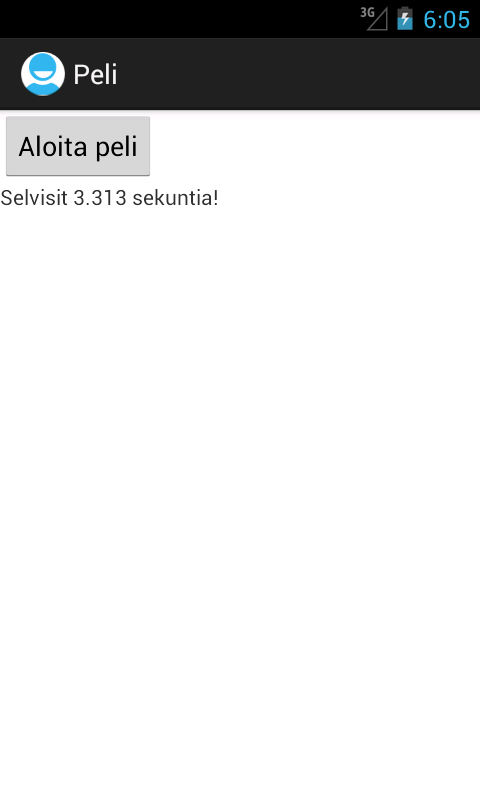
\includegraphics[width=60mm]{peli_mainactivity.png}
\caption{Testiohjelman päänäkymä} \label{mainactivity}
\end{figure}

Peli koostuu kahdesta aktiviteetista, yksinkertaisemmasta MainActivitysta sekä hieman monimutkaisemmasta GameActivitysta, jonka yksikkötestaukseen keskityn. Itse peliä ohjaa GameView-luokka, joka on yhtä aikaa näkymä ja kontrolleri MVC-suunnittelumallin mukaisesti. Malleja ovat GameClock, joka kuvaa pelikelloa, sekä Circle, joka kuvaa yhtä ruudulla näkyvää ympyrää. GameActivity toteuttaa lisäksi OnGameEndListener-rajapinnan, jonka avulla GameView ilmoittaa pelin päättymisestä ja pistemäärästä. Pelin luokkakaavio on esitetty kuvassa \ref{game_classdiagram}.

\begin{figure}[h]
\centering
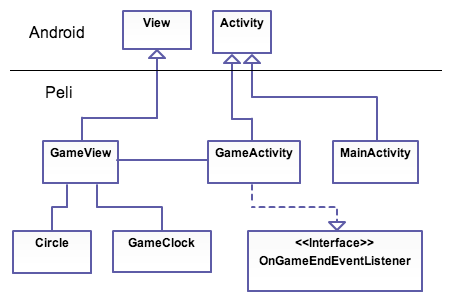
\includegraphics[width=105mm]{peli_luokkakaavio.png}
\caption{Testiohjelman luokkakaavio} \label{game_classdiagram}
\end{figure}

\subsection{Robolectricin asentaminen}
\label{robolectric_install}

Robolectricin suositeltu asennustapa on Maven, joka on yleisesti käytössä oleva kääntämis- ja riippuvuuksienhallintatyökalu \cite{maven}. Koska testattava projekti ei ollut Maven-projekti, jouduin tekemään Robolectric-testitkin ilman Mavenia. Ilman Mavenia asennus osoittautui haastavaksi: eri kirjastopakettien riippuvuudet eivät tahtoneet mitenkään toimia yhteen. Lopulta asennus kuitenkin onnistui tekemällä Robolectricin TestRunnerista oma aliluokka. Listauksessa \ref{robolectric_runner} on muokattu Robolectricin aliluokka testejä varten lähteenä olleesta esimerkistä \cite{sample_runner}. Olennaista on, että yliluokalle syötetään konstruktoriparametrina RobolectricConfig-olio, jolle annetaan parametrina testattavan Android-sovelluksen AndroidManifest.xml sekä resurssi-hakemiston osoite.

\begin{lstlisting}[float,label=robolectric_runner,caption=CustomRobolectricTestRunner]
public class CustomRobolectricTestRunner extends RobolectricTestRunner {
  public CustomRobolectricTestRunner(@SuppressWarnings("rawtypes") Class testClass) throws InitializationError {
  	super(testClass, new RobolectricConfig(new File("../Demo/AndroidManifest.xml"), new File("../Demo/res")));
  }
}
\end{lstlisting}

Robolectric-testejä varten luodaan oma tavallinen Java-projekti Eclipsessä, joka laitetaan viittaamaan Android-projektin koodiin. Testiprojektin käännöspolkuun tarvitaan Robolectricin jar-paketti, sekä Androidin android.jar sekä maps.jar -paketit. Robolectricin paketin pitää olla riippuvuuslistassa ennen Android-paketteja, jotta se toimii. Tämän jälkeen testejä voi ohjelmoida kuten tavallisia JUnit-testejä.

\subsection{Perusominaisuudet}
\label{basic_unittests} 

\begin{lstlisting}[float,label=robolectric_activitytest,caption=Yksinkertainen aktiviteettiyksikkötesti Robolectricilla]
@RunWith(CustomRobolectricTestRunner.class)
public class GameActivityTest {

  private GameActivity activity;

  @Before
  public void setUp() {
    activity = new GameActivity();
    activity.onCreate(null);
  }

  @Test
  public void testActivityInitializesViewWithRunningState() throws Exception {
    GameView gameView = (GameView) activity.findViewById(R.id.gameview);
    assertThat(gameView.getState(), equalTo(GameState.RUNNING));
  }
  
  @Test
  public void testOnPauseStopsTheGame() {
  	activity.onPause();
  	GameView gameView = (GameView) activity.findViewById(R.id.gameview);
  	assertThat(gameView.getState(), equalTo(GameState.PAUSED));
  }
  
}
\end{lstlisting}

Aktiviteetin elinkaarimetodien testaus on olennaisin osa Android-sovellusten yksikkötestauksesta. Listauksessa \ref{robolectric_activitytest} on yksinkertainen aktiviteettiyksikkötesti Robolectricillä toteutettuna. Robolectricin testit ovat yhteensopivia JUnitin 4. version kanssa, mikä mahdollistaa annotaatioiden käytön testeissä. @RunWith-annotaatiolla määritellään testien ajossa käytettävä testiajuri (\emph{runner}). Testissä käytetään luvussa \ref{robolectric_install} esiteltyä ajuria. @Before-annotaatiolla ilmaistaan metodit, jotka on ajettava ennen testejä ja @Test-annotaatiolla ajettavat testit.

setUp()-metodissa alustetaan testattava aktiviteetti ja kutsutaan sen onCreate()-metodia. Robolectric havaitsee automaattisesti Androidin kirjastometodien kutsun ja korvaa ne Robolectricin toteutuksella, jotta ne toimivat testissä. Siksi aktiviteetti voidaan alustaa suoraan konstruktorilla ja kutsua sen onCreate()-metodia toisin kuin AndroidUnitTestissä, jossa aktiviteetti käynnistetään AndroidUnitTestCase-luokan tarjoamien apumetodien avulla.

Ensimmäisessä testissä testataan, että aktiviteetin onCreate()-metodista alustetaan GameView-olio Running-tilaan. Robolectricin toteutus findViewById()-metodista mahdollistaa View-olion löytämisen Android-sovelluksen resursseissa määritellyn tunnisteen perusteella. Tämän jälkeen varmistetaan, että GameViewin tila on todella vaihtunut Running-tilaan. 

Toinen testi on rakenteeltaan hyvin samanlainen: siinä testataan, että onPause()-elinkaarimetodin kutsuminen siirtää GameViewin pause-tilaan. Testimekaniikka on sinänsä täsmälleen samanlainen kuin ensimmäisessä testissä.

Nämä testit eivät vaadi mitenkään ottamaan huomioon, että testejä tehdään Robolectriciä, eikä oikeaa Androidia vastaan. Robolectric toimii taustalla automaattisesti ja mahdollistaa testien vaatimat Androidin kirjastokutsut.

\begin{lstlisting}[float,label=androidunit_activitytest,caption=Yksinkertainen aktiviteettiyksikkötesti ActivityUnitTestCasen avulla]
public class GameActivityTest extends ActivityUnitTestCase<GameActivity> {

  private GameActivity activity;

  public GameActivityTest() {
  	super(GameActivity.class);
  }

  public void setUp() throws Exception {
  	super.setUp();
  	startActivity(new Intent(getInstrumentation().getTargetContext(), GameActivity.class), null, null);
    activity = (GameActivity)getActivity();
  }

  public void testActivityInitializesViewWithRunningState() {
    GameView gameView = (GameView) activity.findViewById(R.id.gameview);
    assertThat(gameView.getState(), equalTo(GameState.RUNNING));
  }
  
  public void testOnPauseStopsTheGame() {
  	activity.onPause();
  	GameView gameView = (GameView) activity.findViewById(R.id.gameview);
  	assertThat(gameView.getState(), equalTo(GameState.PAUSED));
  }
  
}
\end{lstlisting}

Listauksessa \ref{androidunit_activitytest} on toteutettu Androidin omalla yksikkötestikirjastolla vastaavat testit kuin listauksessa \ref{robolectric_activitytest}. Itse testit ovat täysin identtisiä Robolectric-testien välillä, erot ovat alustuksessa. Androidin aktiviteettiyksikkötestit perivät yliluokan ActivityUnitTestCase, jolle annetaan konstruktoriparametrina testattavan aktiviteetin luokka. Tämän jälkeen yliluokka instrumentoi luokan testausta varten.

setUp()-metodissa kutsutaan yliluokan setUp()-metodia ja käynnistetään testattava aktiviteetti yliluokan tarjoamalla startActivity()-metodilla. Tämän jälkeen viite testattavaan aktiviteettiin saadaan yliluokan getActivity()-metodilla.

Robolectricistä poiketen Androidin yksikkötestit ovat JUnit3-pohjaisia, joten annotaatioita ei käytetä, vaan metodien nimien perusteella päätellään setUp()-metodi sekä testimetodit siitä, että niiden nimi alkaa sanalla test. Koska JUnit3-testit kutsuvat testien alustamiseksi nimenomaan setUp()-nimistä metodia, on metodin alussa muistettava kutsua yliluokan setUp()-metodia, tai yliluokan suorittamat alustukset jäävät tekemättä.

\begin{lstlisting}[float,label=robolectric_shadow,caption=Aikeen tilatietojen tarkastelu Robolectricin varjo-olioilla]
@Test
public void testMainActivityIsCalledAfterLostGame() {
  GameView gameView = (GameView) activity.findViewById(R.id.gameview);
  gameView.setState(GameState.LOST);
  	
  ShadowActivity shadowActivity = shadowOf(activity);
  Intent startedIntent = shadowActivity.getNextStartedActivity();
  assertThat(startedIntent.getComponent().getClassName(), equalTo(MainActivity.class.getName()));
  assertThat(startedIntent.getStringExtra(GameActivity.SCORE), equalTo("0.0"));
}
\end{lstlisting}

Listauksessa \ref{robolectric_shadow} on hieman monimutkaisempi testitapaus Robolectricilla samasta testiluokasta kuin listaus \ref{robolectric_activitytest}. Tässä testissä testataan tapahtumia pelin loppuessa. Jos aktiviteetti toimii oikein, se rekisteröi GameView-oliolle havainnoija-suunnittelumallin (\emph{observer}) mukaisen havainnoijan, jota kutsutaan, kun peli päättyy. Aktiviteetin pitäisi tämän jälkeen pyytää GameView-oliolta pistemäärä ja lähettää uusi aie, jolla käynnistetään MainActivity-aktiviteetti ja annetaan aikeelle ylimääräisenä tietona saatu pistemäärä.

Androidin Activity-luokka ei tarjoa suoraa julkista metodia, jolla voitaisiin kysyä, minkä aikeen aktiviteetti on lähettänyt. Tällaisia tapauksia varten Robolectricilla on valmiina varjototeutus, joka kopioi oikean Android-luokan tilan ja tarjoaa laajemman mahdollisuuden aktiviteetin tilan kyselyyn. Tätä varten testissä tehdään varjo-olio testattavasta aktiviteetista, jolloin varjo-oliolta voidaan kysyä getNextStartedActivity()-metodilla, mikä on seuraava käynnistettävä aktiviteetti. Tältä aikeelta voidaan sitten tarkistaa, että aktiviteetti lähetti aikeen MainActivity-aktiviteetin käynnistämiseksi ja ylimääräisenä tietona on pistemäärä. Tässä tapauksessa pisteiden oletetaan olevan 0.0, koska pelikelloa ei missään testin vaiheessa käynnistetty.

\begin{lstlisting}[float,label=android_intent,caption=Aikeen tilatietojen tarkastelu ActivityUnitTestCasen avulla]
public void testMainActivityIsCalledAfterLostGame() {
  GameView gameView = (GameView) activity.findViewById(R.id.gameview);
  gameView.setState(GameState.LOST);
  	
  Intent startedIntent = getStartedActivityIntent();
  assertThat(startedIntent.getComponent().getClassName(), equalTo(MainActivity.class.getName()));
  assertThat(startedIntent.getStringExtra(GameActivity.SCORE), equalTo("0.0"));
}
\end{lstlisting}

Listauksessa \ref{android_intent} on toteutettu vastaava testi AndroidUnitTestCase:n avulla. Alustus tehdään testissä kuten Robolectric-testissäkin, mutta toiminnan varmistus on yksinkertaisempaa kuin Robolectricillä, koska AndroidUnitTestCase tarjoaa getStartedActivityIntent()-metodin, jolla saadaan aktiviteetin viimeisin lähettämä aie palautettua samalla tavalla kuin Robolectricin varjo-oliolta kysyttiin edellisessä listauksessa. Tämän jälkeen testin läpipääsyn varmistus tapahtuu täsmälleen samalla tavalla kuin Robolectric-testissä.

\subsection{Toiminta jäljittelijäkehysten kanssa}

Yksikkötestausta pyritään useimmiten tekemään niin, että testiluokka on eristetty riippuvuuksistaan. Apuvälineenä eristämisessä käytetään usein jäljittelijäkehyksiä. Näissä testeissä jäljittelijäkehyksenä käytetään Mockitoa, koska se toimii myös Androidissa sellaisenaan \cite{mockito}. Emulaattorissa ajamiseen tarvitsee vain Dalvik-käännöspaketin

Luvussa \ref{basic_unittests} esitetyt yksikkötestit ovat riippuvaisia GameView-luokan toteutuksesta. Testit voivat kuitenkin palauttaa virheellisen tuloksen, jos GameView-luokan setState()-metodi ei muutakaan onnistuneesti tilaa. Tällöin kyse on kuitenkin GameView-luokan, eikä GameActivity-luokan toiminnasta. GameActivityn osalta testissä ollaan oikeastaan vain kiinnostuneita siitä, että aktiviteetin käynnistyessä pelin tilaa yritetään muuttaa RUNNING-tilaan.

\begin{lstlisting}[float,label=mock_subclass, caption=Jäljittelijäaliluokka]
private class MockGameActivity extends GameActivity {
	
	private GameView gameView;

  public MockGameActivity(GameView gameView) {
	  setView(gameView);
  }

  @Override
  public View findViewById(int id) {
	  return gameView;
  }
  
  public void setView(GameView gameView) {
    this.gameView = gameView
  }
}
\end{lstlisting}

Aktiviteetti on testissä eristettävä GameView:stä niin, että oikean näkymän sijaan se saa käyttöönsä jäljitellyn version näkymästä. Aktiviteetti käyttää findViewById()-metodia näkymän lataamiseen, koska se on alustettu layout-tiedostossa. Jotta tähän metodikutsuun pääsee väliin, täytyi aktiviteetille tehdä testiä varten aliluokka MockGameActivity, joka on esitetty listauksessa \ref{mock_subclass}. Aliluokka toteuttaa findViewById()-metodista version, joka palauttaa aina sille parametrina annetun näkymän, joka voi olla esimerkiksi jäljitelty näkymä. Tämä on yleinen tapa käyttää jäljittelijäkehyksiä riippuvuuksien eristämiseksi.

Tämän voisi Robolectricillä tehdä vaihtoehtoisesti siten, että toteuttaa oman varjoluokan Activity-luokasta, joka on kaikkien aktiviteettien yliluokka. Toteutuksen voi tehdä siten, että käyttää Robolectricin oletustoteutusta kaikkeen muuhun paitsi findViewById()-metodin toteutukseen \cite{robolectric}. Jäljittelijänäkymän injektointia varten tälle voisi tehdä myös oman set-metodin, jolla jäljitelty näkymä sijoitettaisiin palautettavaksi. Yllä esitetty testattavan luokan aliluokka on kuitenkin helpompi tapa toteuttaa sama asia, koska Robolectriciä ei tarvitse erikseen käskeä käyttämään varjoluokkana itse tehtyä toteutusta. Lisäksi aliluokkatoteutuksella on helpompi vaihdella, käytetäänkö testeissä oman aliluokan ilmentymää, vai varsinaisen testattavan luokan ilmentymää.

\begin{lstlisting}[float,label=mock_test_robolectric, caption=Jäljittelyä käyttävä testi Robolectrcicillä]
@Test
public void testActivityInitializesGameWithRunningStateWithMock() throws Exception {
	GameView gameView = mock(GameView.class);
	activity = new MockGameActivity(gameView);
	activity.onCreate(null);
	verify(gameView).setState(GameState.RUNNING);
}
\end{lstlisting}

Listauksessa \ref{mock_test_robolectric} on esitetty edellisen listauksen aliluokkaa käyttävä Robolectric-testi. Ensimmäisellä rivillä luodaan Mockiton jäljittelijäolio GameView-luokasta. Toisella rivillä luodaan testattavan aktiviteetin aliluokka, jolle syötetään jäljitelty näkymä konstruktoriparametrina. Sitten kutsutaan onCreate-metodia, kuten listauksen \ref{robolectric_activitytest} vastaavassa testissä. Testin läpäisy testataan Mockiton verify-metodilla, joka varmistaa, että parametrina annettua jäljittelijäolion annettua metodia kutsuttiin annetulla parametrillä.

\begin{lstlisting}[float,label=mock_test_android, caption=Jäljittelyä käyttävä testi AndroidUnitTestillä]
public void testActivityInitializesGameWithRunningStateWithMock() throws Exception {
	GameView gameView = mock(GameView.class);
	MockGameActivity.setView(gameView);
	startActivity(new Intent(getInstrumentation().getTargetContext(), MockGameActivity.class), null, null);
	verify(gameView).setState(GameState.RUNNING);
}
\end{lstlisting}

AndroidUnitTestin avulla tehty vastaava testi listauksessa \ref{mock_test_android} on jäljittelijänäkymän luomisen ja testin läpäisyn varmistamisen kannalta täsmälleen samanlainen kuin Robolectric-testi. Testissä käytetään apuna vastaavaa aliluokkaa kuin Robolectric-testissäkin, mutta näkymä pitää syöttää aliluokalle setView()-metodissa, koska AndroidUnitTestille annetaan testattavan luokan nimi jo luokan määrittelyssä ja aktiviteetti käynnistetään yliluokan avulla jo ennen testeihin pääsyä.

\subsection{Testisyklin nopeus}

Robolectricin vahvuudeksi mainitaan toistuvasti sen testien ajonopeus. Testien ajonopeudella on merkitystä kahdesta syystä: ensinnäkin laajojen projektien tapauksessa testitapauksia voi olla hyvin paljon ja kaikkien testien ajo voi kestää hyvin pitkään, mikä hidastaa koodin jakamista tai ohjelmistotuotantoprosessia, kun muutosten regressiotestaus aiemmin tehtyjen yksikkötestien avulla kestää pitkään. Toiseksi kehitettäessä sovellusta esimerkiksi Mobile-D-prosessin mukaisesti testilähtöisesti osaa testejä ajetaan jatkuvasti. Prosessi pysähtyy aina testien ajoajaksi, joten jos yksittäisten testien ajaminen on kovin hidasta, ei testilähtöinen kehittäminen ole järkevää.

\begin{table}[h]
\centering
\begin{tabular}{ l l l l }
   & Keskiarvo (s) & Max (s) & Min (s) \\
  Robolectric & 1,59 & 1,61 & 1,577 \\
  AndroidUnitTest & 44,10 & 44,271 & 43,868 \\
\end{tabular}
\caption{Testisarjan kestot Robolectricilla ja AndroidUnitTestillä}
\label{unittest_timing}
\end{table}

Testasin ensin isomman testisetin ajonopeutta. Kopioin aiemmin luvussa esitellyn testiluokan jäljittelijätestin kanssa 32 erilliseksi testiluokaksi niin, että testimetodeita kertyi yhteensä 128. Ajoin kaikki testit yhtenä sarjana ja annoin Eclipsen ottaa aikaa testien suorituksesta. Tähän aikaan ei sisälly sitä aikaa, joka kuluu JUnitin käynnistymiseen, vain itse testien suoritusaika. Toistin testit viisi kertaa ja testikestojen keskiarvo, maksimi ja minimi on esitetty taulukossa \ref{unittest_timing}. Testit ajoin Macbook Pro:lla OS X versiolla 10.7.5, joka oli varustettu 2,7Ghz Intel core i7 -tuplaydinprosessorilla ja 8 gigatavun muistilla.

Robolectricin testit kestivät keskimäärin 1,59 sekuntia, AndroidUnitTestilla 44,10 sekuntia. Testien ajaminen emulaattorissa oli siis noin 27 kertaa hitaampaa kuin Robolectricilla JVM:llä. Koska testattava sovellus ja itse testit ovat hyvin yksinkertaisia, on aikaero todennäköisesti vielä suurempi laajempaa sovellusta testattaessa. Robolectricin lupaus nopeammista yksikkötesteistä vaikuttaa siis toteutuvan.

Testisarjan keston lisäksi tutkin yksittäisten testien kestoja. Erityisen kauan emulaattorissa ajetuista testeistä kesti ensimmäisen testiluokan jäljittelijätesti. Sen ajo kesti jokaisella ajokerralla yli 12 sekuntia, eli yli 25\% koko testisarjan kestosta. Tämä johtuu siitä, että Mockito muokkaa ohjelman tavukoodia toimintaansa varten ja sen ensimmäinen alustus on hyvin hidas. Sama hitaus oli havaittavissa myös Robolectric-testeissä: ensimmäinen mock-testi kesti noin 0,3 sekuntia, mikä on noin 19\% koko Robolectric-testisarjasta. Suhteellinen hidastuminen on siis verrattavissa AndroidUnitTestillä ajettuihin testeihin.

Robolectricillä myös kaikkein ensimmäinen testi on suhteessa hyvin hidas, noin 0,5 sekuntia. Robolectric toimii tavukooditason muokkauksessa Mockiton tavoin instrumentoidessaan testattavaa sovellusta toimimaan Robolectricin varjototeutusten kanssa, joten ensimmäisen testin suhteellinen hitaus johtunee samasta syystä kuin Mockitolla.
Nämä seikat eivät kuitenkaan muuta kokonaiskuvaa siitä, että testien ajaminen on todella paljon nopeampaa Robolectricillä kuin AndroidUnitTestillä.

\begin{table}[h]
\centering
\begin{tabular}{ l l l }
   & Ensimmäisen testin alkuun (s) & Koko testisarjan loppuun \\
  Robolectric & 2,7 & 4,3 \\
  AndroidUnitTest & 36 & 80 \\
\end{tabular}
\caption{Testisarjan kesto alustus mukaanlukien}
\label{unittest_startup}
\end{table}

Toiseksi testasin, kuinka kauan kestää testikehyksen alustus siihen pisteeseen, että ensimmäinen testi lähtee ajautumaan koodimuutoksen jälkeen. Tämä tarkoittaa Android-tapauksessa sovelluksen asentamista emulaattoriin ja testikehyksen alustusta. Tulokset on esitetty taulukossa \ref{unittest_startup} Alustusajat olivat merkittäviä. Robolectricillä testikehyksen alustus kestää jopa kauemmin kuin koko 128 testin sarjan ajo ja AndroidUnitTestilläkin lähes yhtä kauan. Yhdenkin testin ajaminen AndroidUnitTestillä kestää yli 30 sekuntia.

\subsection{Yksikkötestauksen haasteita}

\begin{lstlisting}[float, label=tomdroid_example,caption=Tomdroid-koodiesimerkki]
public class EditNote extends ActionBarActivity {
  ...
  protected void onCreate(Bundle savedInstanceState) {
    ...
    content = (EditText) findViewById(R.id.content);
    ...
    Intent intent = getIntent();
    uri = intent.getData();
  }  
  
  public void onResume(){
    ...
    if (uri == null) {
  	  ...
    } else handleNoteUri(uri);
  }

  private void handleNoteUri(final Uri uri) {
    ...
    note = NoteManager.getNote(this, uri);
    if(note != null) {
      noteContent = note.getNoteContent(noteContentHandler);
    }
  }
  
  private Handler noteContentHandler = new Handler() {
    ...
    public void handleMessage(Message msg) {
      ...
      if(msg.what == NoteContentBuilder.PARSE_OK) {
      	showNote(false);
      	...
      }
      ...
    }
  }
  
  private void showNote(boolean xml) {
    ...
    content.setText(noteContent, TextView.BufferType.SPANNABLE);
    ...
  }
}
\end{lstlisting}

Koodin laadun suhteen yksikkötestaus on herkkää: alunperin tarkoitukseni oli tehdä yksikkötestaus luvussa \ref{tomdroid} esiteltyä sovellusta vasten kuten toiminnallinen testauskin. Tämä ei kuitenkaan onnistunut, koska sovellusta ei ollut mitenkään tehty yksikkötestaus mielessä, osoittautui tämä mahdottomaksi.

Aloitin yrittämällä testata muistikirjan muokkausnäkymässä, että aktiviteetin käynnistys lataa muistikirjan sisällön. Listauksessa \ref{tomdroid_example} näkyy EditNote-aktiviteetin koodi, joka liittyy muistikirjan sisällön asettamiseen. onCreate()-metodin sisältö on suoraviivainen: content-muuttuja alustetaan ja aikeelta pyydetään uri, joka on muistikirjan tunniste. onResume()-metodissa kutsutaan yksityistä handleNoteUri()-metodia. Tässä metodissa pyydetään muistikirja NoteManagerin staattisella getNote()-metodilla ja jos muistikirja löytyy, pyydetään muistikirjalta sen sisältö getNoteContent()-metodilla, joka ottaa parametrikseen käsittelijän, joka on EditNoten yksityinen sisäluokka. 

Tässä kohdassa aktiviteetti muuttuu mahdottomaksi testata eristettynä riippuvuuksistaan. Ensimmäinen ongelma on staattinen NoteManager, jota ei voi suoraan jäljitellä Androidissa toimivilla jäljittelijäkehyksillä. Tämä ongelma on kuitenkin kierrettävissä vähäisellä ohjelmakoodimuutoksella: kääritään staattinen kutsu EditNoteen tehtävään uuteen metodiin getNote(), joka voidaan sitten jäljitellä testissä jäljittelyaliluokassa kuten listauksessa \ref{mock_subclass} tehtiin.

Lopullinen este testaamiselle on kuitenkin kohta, jossa muistikirjalta pyydetään sen sisältö getNoteContent()-metodilla. Metodi toimii siten, että sille annetaan parametriksi käsittelijä, joka on EditNoten yksityinen sisäluokka. Tämän käsittelijän sisältä handleMessage()-metodista taas kutsutaan showNote()-metodia, joka asettaa tekstin käyttöliittymään. Onnistuin jäljittelemään tämänkin toiminnan siten, että Note-olio oli jäljitelty ja sen getNoteContent()-tyngästä kutsuttiin parametrina annetun käsittelijän handleMessage()-metodia. Tässä vaiheessa testi kaatui, koska oikeasti getNoteContent()-metodi on asynkroninen ja getNoteContent()-metodin palauttama noteContent ehditään asettaa ennen kuin käsittelijästä kutsutaan showNote()-metodia. Tässä vaiheessa yksinkertaista testiä varten oli kertynyt jäljittelijäkoodia useita kymmeniä rivejä ja totesin testaamisen epäkäytännölliseksi.

Tämä osoittaa, että ohjelmakoodin täytyy olla rakenteeltaan kelvollista ja luokkien ja metodien noudattaa mahdollisimman pitkälti yhden vastuun periaatetta (\emph{single responsibility principle}, ks. \cite[95-98]{agile_development}), jotta niiden yksikkötestaus on mahdollista. Lisäksi suurin hyöty yksikkötesteistä on ennen ohjelmakoodia kirjoitettuna, jolloin myös koodin rakenne pysyy helpommin testattavana.

\subsection{Analyysi}

Ohjelmakoodin yksikkötestaus onnistui hyvin sekä Androidin mukana tulevalla yksikkötestikehyksellä, että Robolectricillä. Itse testikoodi ei poikennut kovin merkittävästi toisistaan eri kehyksille kirjoitetulla koodilla ja testien kirjoitukseen ei tarvinnut kovin paljoa Android-spesifiä osaamista. Robolectric-koodi oli jopa yksinkertaisempaa testattavien komponenttien alustuksen ostalta, koska konstruktoreja saattoi käyttää suoraan yliluokan tarjoamien alustusmetodien sijaan. Toisaalta joskus oli vaikea tietää, mitä metodeita eri luokkien valmiit varjototeutukset tarjoavat. Näissä tapauksissa AndroidUnitTestCasen yliluokkametodit olivat käytössä selkeämpiä. Toisaalta Robolectric tarjoaa mahdollisuuden kirjoittaa itse omia varjoluokkia, joissa voi toteuttaa tynkiä Androidin kirjastoluokkien toiminnalle.

Jäljittelijäkehyksen käyttö onnistui ongelmitta sekä Robolectricillä että AndroidUnitTestCasella. Mockito toimi suoraan yhdessä Robolectricin kanssa ja Android-emulaattorissa ajaminenkin onnistui helposti.

Suurin ero testityökalujen välillä oli testien suoritusnopeudella. Robolectric lupaa nopeita testejä ja toteuttaa lupauksensa; Robolectric-testit ajautuivat yli 25 kertaa nopeammin kuin emulaattorissa ajetut AndroidUnitTestit. Lisäksi AndroidUnitTestillä aika ensimmäiseen testitulokseen pienelläkin testiohjelmalla oli yli puoli minuuttia, joten testilähtöinen ohjelmointi AndroidUnitTestCasea käyttäen on käytännössä toivottoman hidasta.

Tässä luvussa testattu sovellus oli hyvin yksinkertainen, joten jotkin tulokset eivät välttämättä skaalaudu suoraan suurempien sovellusten testaamiseen. Toisaalta yksikkötestauksessa pyritään yleensä riippuvuuksien rajaamiseen ja mahdollisimman pienten osien testaamista erikseen, joten periaatteessa suurempien sovellusten yksikkötestaaminen ei ole juuri vaikeampaa kuin yksinkertaisten. 

Toinen kysymys on ylipäänsä aktiviteettien yksikkötestauksen mielekkyys. Hyvin rakennetussa sovelluksessa sovelluslogiikka on eriytetty käyttöliittymälogiikasta omiin luokkiinsa, joten sovelluslogiikan yksikkötestaus onnistuu myös tavallisella JUnitilla. Sovelluslogiikassa useimmiten on myös testauksen kannalta tärkeimmät osat. Käyttöliittymälogiikan yksikkötestausta tehokkaampaa voisi sen sijaan olla suora toiminnallinen testaus käyttöliittymän kautta.
\clearpage
\section{Toiminnallinen testaus}

Robotium, Troyd, Uiautomator ja ehkä myös monkeyrunner?

\subsection{Robotium}

Robotium ei tule Androidin sdk:n mukana, mutta se on paljon käytetty testityökalu Android-sovellusten testauksessa. Robotiumin slogan on, että se on kuin Selenium, mutta Androidille. Selenium taas on laajasti integraatio- ja funktionaalisessa testauksessa käytetty työkalu, joka mahdollistaa selaimen toimintojen automatisoimisen, kuten linkkien klikkauksen, lomakekenttien täyttämisen jne. \cite{selenium}

Robotium on tarkoitettu Android-sovellusten funktionaaliseen-, systeemi- ja hyväksyntätestaukseen. Se on black box -työkalu, eli testin kirjoittajan ei tarvitse päästä käsiksi tai tuntea testattavan sovelluksen koodia. Robotium-testit voivat testata samassa testitapauksessa useita aktiviteetteja. Robotium-testeissä annetaan ohjeita, missä järjestyksessä käyttöliittymäelementtejä klikataan tai syötetään tekstiä.

Robotiumtestejä voi ajaa niin emulaattorissa kuin puhelimessakin. Testit eivät kuitenkaan voi käsitellä kahta eri sovellusta, eli yksi testitapaus voi käsitellä vain yhtä sovellusta. Tällöin sovellustenvälinen integraatiotestaus ei ole mahdollista.

Robotiumin sivuilla sille esitellään useita vahvuuksia Android SDK:n mukana tuleviin työkaluihin verrattuna. Testit vaativat vain vähäistä tuntemusta testattavasta sovelluksesta, Robotium tukee usean aktiviteetin testaamiseta samassa testissä, testien kirjoittamisen nopeus, testikoodin selkeys ja sitkeys, joka johtuu ajoaikaisesta sidonnasta käyttöliittymäkomponentteihin, nopea suoritusnopeus ja helppo integrointi jatkuvan integroinnin työkaluihin Antin tai Mavenin avulla. (pitäisikö ant/maven esitellä jossain?) \cite{robotium}

\subsection{Troyd}

Troyd on Robotiumia käyttäen tehty integraatiotestaustyökalu, jonka tavoite on yhdistää Monkeyn skriptausominaisuudet ja Robotiumin tarjoama korkean tason API. Troyd-testit käyttävät korkean tason komentoja, kuten paina nappia nimeltä x, tarkista, että ruudulla näkyy teksti y, jne, joten testien kirjoituksen pitäisi olla nopeaa. Lisäksi Troyd tarjoaa nauhoitus-toiminnon, jolla testiä voidaan kirjoittaa siten, että testiä kirjoittaessa ohjelma etenee aina seuraavaan tilaan testin mukaisesti. Lopuksi testi tallentuu testitapauksiksi. \cite{troyd}

Troyd-testejä kirjoitetaan Rubylla käyttäen Rubyn Test::Unit-työkalua, joka on Rubyn standardi yksikkötestityökalu. \cite{testunit} Troydin komennot sisältävä TroydCommands-moduli sisällytetään testiluokkaan käyttämällä Rubyn mixin-toiminnallisuutta. Testitapauksia voi kirjoittaa kuten tavallisia test::unit-testejä tai sitten voi käyttää rec-skriptin nauhoitusmahdollisuutta.

Troydin heikkouksia on Jeonin ja Fosterin mielestä mahdollisuus testata vain yhtä sovellusta kerrallaan. Esimerkiksi, jos sovellus aukaisee selainikkunan, Troyd menettää sovelluksen kontrollin. Tämä johtuu Androidin testi-instrumentaation rajoituksista. Toinen Troydin heikkous on hidas suoritusnopeus, koska testiskripti odottaa jokaisen komennon jälkeen, että sovellus on oikeassa tilassa ennen testin jatkamista. \cite{troyd}

Troydin lähdekoodi on avoin ja se löytyy Githubista \cite{troyd_github}.

\subsection{Aiempaa tutkimusta}

Jeon \& Foster mainitsevat Robotiumin vahvuudeksi Androidin omaa Instrumentatiota rikkaamman APIn. Esimerkiksi nappien painamiseen voidaan käyttää nappien nimeä, josta Robotium laskee napin sijainnin. He myös vertaavat Robotiumia omaan Troyd-työkaluunsa ja sanovat sen heikkoudeksi, että testit pitää määritellä etukäteen, eikä niitä pysty muokkaamaan ajonaikaisesti. Muulta toiminnallisuudeltaan Troyd ja Robotium ovat suunnilleen samankaltaisia, koska Troyd on tehty Robotiumin päälle \cite{troyd}.

Benli et al. tutkivat valkoinen laatikko ja musta laatikko -testaustapojen suhteellista tehokkuutta Android-alustalla. Musta laatikko -testeissä tutkimuksessa käytettiin Robotiumia, koska Androidin mukana tulevat testaustyökalut eivät mahdollistaneet järkevää JUnit-pohjaista musta laatikko -testausta. Valkoinen laatikko -testit tehtiin Androidin yksikkötestityökaluilla. Tuloksena oli, että valkoinen laatikko -testien kirjoittaminen kesti 89\% kauemmin, mutta testien ajaminen oli 43\% nopeampaa kuin musta laatikko -testien. Testiohjelmaan istutetut bugit löytyivät valkoinen laatikko -testeillä, mutta ei Robotium-testeillä. Testiajojen nopeuteen liittyen on huomattava, että robotium-testit ajettiin visuaalisessa moodissa niin, että jokaisen komennon välissä oli yksi sekunti, jotta käyttöliittymän tila ehdittiin havaita manuaalisesti \cite{benli12}.

\subsection{Testiprojektista}

\begin{figure}[htb]
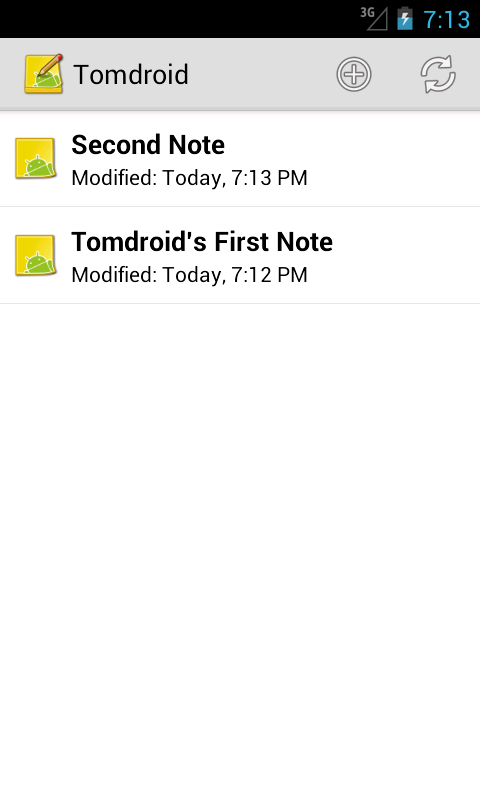
\includegraphics[width=60mm]{tomdroid_notelist.png}
\caption{Muistikirjalista Tomdroidissa} \label{tomdroid_notelist}
\end{figure}

Testityökalujen vertailussa käytän testattavana ohjelmana Tomdroidia. Tomdroid on GPL-lisenssillä julkaistu avoimen lähdekoodin sovellus, joka toimii muistikirjasovelluksena, joka synkronisoi sisältönsä automaattisesti. \cite{tomdroid} Tomdroid on valittu testattavaksi sovellukseksi, koska sen lähdekoodi on saatavilla, se on riittävän monimutkainen, jotta sille tehdyt testit kuvaisivat oikeassa android-kehityksessä kohdattavia testaushaasteita, se on vasta beta-vaiheessa, joten sovelluksesta pitäisi löytyä myös bugeja ja lisäksi sovelluksen oma testaus on lähes olematonta.

Tätä tutkimusta varten tein kopion tomdroidin lähdekoodista versiosta 0.7.2 ja kopioin sen githubiin. Sieltä löytyy myös kaikki tässä tutkimuksessa sovellukselle tehdyt testit. \cite{tomdroid_github}

Tomdroidissa olennaisimmat näkymät ovat muistikirjalista, josta on ruutukaappaus kuvassa \ref{tomdroid_notelist}, yksittäisen muistikirjan selaaminen (kuvassa \ref{tomdroid_noteview}) ja sen editointi (kuvassa \ref{tomdroid_editview}). 

Listanäkymässä näkyvät kaikki käyttäjän muistikirjat päivitysajan mukaan järjestettynä. Muistikirjan koskeminen avaa kyseisen muistikirjan selausnäkymän. Yläpalkin +-symboli luo uuden muistikirjan ja avaa sen editointinäkymään. Yläpalkin oikeassa reunassa on synkronointi-symboli, josta muistikirjojen tila päivitetään palvelimen kanssa.

Selausnäkymässä voi lukea yksittäistä muistikirjaa. Jos tekstiä on enemmän kuin ruudulle mahtuu kerrallaan, sitä voi selata raahaamalla. Kynä-ikoni yläpalkissa avaa muistikirjan editointinäkymään. Yläpalkin oikean reunan ikonista voi jakaa muistikirjan toisiin sovelluksiin. Lisäksi vasemman yläreunan ikonista pääsee takaisin listaan.

Editointinäkymässä yläpalkissa on kuvakkeet muutosten tallentamista ja perumista varten. Tallennettaessa ruudulla näkyy hetken aikaa leijuke, jossa kerrotaan muutosten tallennuksesta. Painettaessa peru-nappia ruudulle tulee dialogi, jossa pitää vahvistaa peruminen edelliseen tallennettuun versioon. Lisäksi vasemman yläreunan ikonista pääsee takaisin listaan.

\begin{figure}[htb]
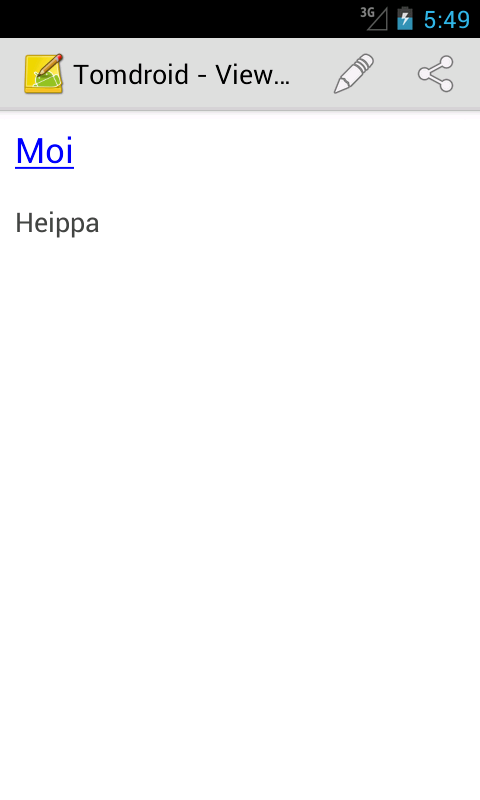
\includegraphics[width=60mm]{tomdroid_noteview.png}
\caption{Muistikirjan luku Tomdroidissa} \label{tomdroid_noteview}
\end{figure}

\begin{figure}[htb]
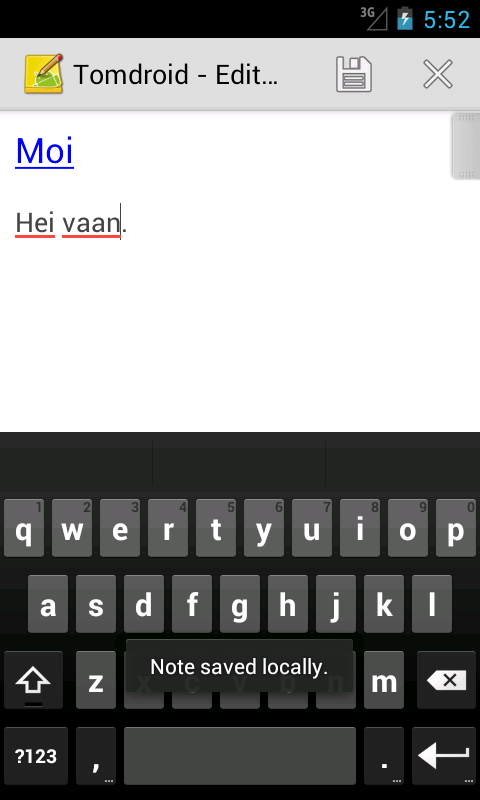
\includegraphics[width=60mm]{tomdroid_editview.png}
\caption{Muistikirjan editointi Tomdroidissa} \label{tomdroid_editview}
\end{figure}

\subsection{Asennukset}

\begin{lstlisting}[float,label=robotium_setup,caption=Robotium testirunko]
public class RobotiumTest 
       extends ActivityInstrumentationTestCase2<Tomdroid> {

	private Solo solo;
	
	public RobotiumTest() {
		super(Tomdroid.class);
	}
	
	@Override
	public void setUp() {
		solo = new Solo(getInstrumentation(), 
		                getActivity());
	}
	
	@Override
	public void tearDown() throws Exception {
		solo.finishOpenedActivities();
	}
}
\end{lstlisting}

Robotiumin asennus on yksinkertaista. Projektin build pathiin tarvitsee vain lisätä robotiumin jar-paketti, jossa tulee kaikki tarvittava mukana. Itse robotium-testit perivät Androidin omasta ActivityInstrumentationTestCase2-yliluokasta. Listauksessa \ref{robotium_setup} on esitetty Robotium-testin runko ilman varsinaisia testejä. setUp()-metodissa alustetaan Solo, joka on Robotiumin testit suorittava olio. Se ottaa konstruktoriparametreina ActivityInstrumentationTestCase2:n tarjoaman instrumentaation ja testattavan aktiviteetin. tearDown()-metodissa kutsutaan finishOpenedActivities()-metodia, joka lopettaa kaikki testin aikana aktiivisena olleet aktiviteetit.

\begin{lstlisting}[float,label=delete_notes,caption=Muistikirjojen poisto]
private void removeAllNotes() {
	NoteManager.deleteAllNotes(getActivity());
}
\end{lstlisting}

Robotium-testeissä on huomattava, että jos sovellus muuttaa muistikortille tai muualle tallennettua tilaansa, on testeissä manuaalisesti pidettävä huolta, että sovellus resetoidaan takaisin alkuperäiseen tilaan, jotta testejä voi toistaa useita kertoja luotettavasti. Tomdroidin tapauksessa tämä tehtäisiin kutsumalla tearDown():ssa apumetodia removeAllNotes(), joka kutsuu Tomdroidin NoteManagerin deleteAllNotes()-metodia, joka poistaa kaikki sovelluksen tallentamat muistikirjat.

\begin{lstlisting}[float, label=troyd_run, caption=Troyd-nauhoitusskriptin ja testien ajaminen]
ruby bin/rec.rb apks/org.tomdroid.apk
ruby bin/trun.rb
\end{lstlisting}

Troyd vaatii toimiakseen Rubyn version 1.8.7 sekä nokogiri-xml-kirjaston. Lisäksi se tukee vain Androidin versiota 2.3.6, joten uudemman Android-version vaativien sovellusten testaaminen ei ole sillä mahdollista. Troydin asennus kesti huomattavasti Robotiumin asennusta kauemmin, vaikka koneellani oli valmiiksi asennettuna Rubyn versionhallintatyökalu rvm \cite{rvm}, jolla oikean ruby-version asennus onnistuu yhdellä komennolla. Rubyn versio 1.8.7 on myös varsin vanha rubyn versio (julkaistu kesällä 2008 \cite{ruby_187}), joten joissain järjestelmissä näin vanhan version asennus voi olla haasteellista. Asennusten jälkeen Troydin testin kirjoittaminen onnistui kuitenkin nopeasti nauhoitus-skriptin avulla, joka hoiti kaiken muun kuin itse testikoodin kirjoittamisen. Nauhoitus ja ajoskriptit listauksessa \ref{troyd_run}. rec.rb on nauhoitusskripti, jolla testit kirjoitetaan ja trun.rb ajoskripti, joka ajaa oletuksena kaikki testcases-hakemistosta löytyvät testit. Testit voivat olla myös eri sovelluksille, jolloin Troyd asentaa kunkin testattavan sovelluksen erikseen.

\begin{lstlisting}[float, label=uiautomator_run,caption=Uiautomator-testien ajaminen]
#!/bin/sh
ant build
adb push bin/TomdroidUiAutomatorTest.jar /data/local/tmp/
adb shell uiautomator runtest TomdroidUiAutomatorTest.jar 
    -c org.tomdroid.test.UiAutomatorTest
\end{lstlisting}

Ui Automator vaatii vähintään androidin api-version 16, jonka mukana tulee uiautomator.jar-paketti, joka täytyy asettaa testiprojektin riippuvuuksiin android.jar:n ja junit3:n ohella. Lisäksi testien ajaminen vaatii tietokoneessa kiinni olevan android-laitteen, johon testattava sovellus (tai sovellukset) on asennettuna. Testien kääntäminen ja ajaminen on esitetty listauksessa \ref{uiautomator_run}. Testit käännetään Apache Antilla \cite{ant}, joka on avoin käännöstyökalu Java-sovellusten kääntämiseen. Toisella rivillä käytetään androidin mukana tulevaa adb-työkalua (Android debug bridge) käännetyn testisovelluksen siirtämiseen puhelimeen ja kolmannella rivillä ajetaan testisovelluksesta luokka org.tomdroid.test.UiAutomatorTest.

\subsection{Robotium-testit}

\begin{lstlisting}[float,label=robotium_createnote,caption=Muistikirjan luontitesti robotiumilla]
public void testCreateNoteAddsNote() {
	solo.assertCurrentActivity("Testi alkoi väärästä aktiviteetista", Tomdroid.class);
	assertFalse(solo.searchText("new note"));
	solo.clickOnActionBarItem(R.id.menuNew);
	solo.assertCurrentActivity("Uuden muistikirjan luonti ei avannut uutta muistikirjaa editointinäkymään", EditNote.class);
	solo.enterText(0, "new note");
	solo.clickOnActionBarItem(R.id.edit_note_save);
	solo.clickOnActionBarHomeButton();
	solo.assertCurrentActivity("Koti-näppäimen painaminen ei vienyt takaisin muistikirjalistaan", Tomdroid.class);
	assertTrue(solo.searchText("new note"));
}
\end{lstlisting}

Robotium-testi, jossa testataan uuden muistikirjan luonti, on esitetty listauksessa \ref{robotium_createnote}. Robotiumilla testiä ohjataan Solo-luokan instanssin kautta, jossa on sovelluksen kanssa kommunikointiin tarkoitettuja metodeja, sovelluksen tilasta kertovia metodeja, sekä assertteja. Testin ensimmäisellä rivillä käytetään assertCurrentActivity()-metodia asserttia varmistamaan, että testi alkaa muistikirjalistasta. Toisella rivillä varmistetaan, että testissä luotavaa muistikirjaa ei vielä löydy listasta. Ilman tätä testissä ei voisi olla varma, että muistikirja on luotu onnistuneesti juuri testin aikana. Seuraavalla rivillä painetaan yläpalkin uuden muistikirjan luovaa nappia clickOnActionBarItem()-metodilla. Se ottaa parametrina komponentin id:n, johon ollaan painamassa. Tämän jälkeen pitäisi avautua uusi muistikirja editointinäkymään, mikä varmistetaan seuraavalla rivillä. Sitten syötetään enterText()-metodilla uuden muistikirjan otsikoksi \"new note\". Ensimmäinen parametri kertoo, monenteenko ruudulla näkyvään tekstinmuokkauskomponenttiin teksti syötetään. Tämän jälkeen klikataan yläpalkin tallennus-nappia ja sitten muistikirjalistaukseen vievää nappia. Lopuksi vielä varmistetaan, että palattiin takaisin muistikirjalistaan ja listasta löytyy nyt juuri luotu aktiviteetti.

\subsection{Troyd-testit}

\begin{lstlisting}[float, label=troyd_createnote,caption=Muistikirjan luontitesti Troydilla]
def test_"create note adds note"
  click "OK"
  assert_not_text "new note"
  clickImg 1
  edit 0, "new note"
  clickImg 1
  clickImg 0
  assert_text "new note"
end
\end{lstlisting}

Troyd-testi, jossa luodaan muistikirja, on esitetty listauksessa \ref{troyd_createnote}. TROYD-testit asentavat aina ensimmäisenä uuteen emulaattoriin koko sovelluksen, joten robotium-testissä tarvittuja vanhojen muistikirjojen poistoa ei tarvita. Tein testin Troydin nauhoitusskriptin avulla, joten itse testi on automaattisesti kirjoitettu tämän pohjalta. Testitiedosto sisältää testimetodin lisäksi metodit sovelluksen alustamiselle ja lopettamiselle sekä testeissä käytetyt ruby-metodit, mutta nämä kaikki TROYD tuotti automaattisesti nauhoitusskriptin avulla. Itse testimetodin sisältö on sama kuin testiskriptissä kirjoittamani komennot. Lisäksi näin sovelluksen testiä vastaavassa tilassa emulaattorissa testiä kirjoittaessa, mikä helpotti testin kirjoittamista. Listauksessa on lisäksi huomautettava, että Rubyssa metodien sulut ovat vapaaehtoiset, mikäli sekaantumisen vaaraa ei ole, siksi testissä metodien parametrit eivät ole sulkujen sisällä. Kun nauhoitusskriptissä on saanut haluamansa testitapauksen valmiiksi, se tallennetaan sofar-metodilla, jonka parametrina on testin nimi, kuten on tehty listauksessa \ref{troyd_record_save}. Finish-komento lopettaa nauhoitusskriptin.

\begin{lstlisting}[float, label=troyd_record_save,caption=Testin tallennus nauhoitusskriptistä Troydilla]
sofar "create note adds note"
finish
\end{lstlisting}

Testin ensimmäisellä rivillä painetaan OK-nappia, koska sovellus näyttää ensimmäisellä käynnistyskerralla ohje-tekstin. Troydilla ei voi varmistaa, missä aktiviteetissa ollaan, kuten Robotium-testissä tehtiin, joskin listan tähän mennessä vierailluista aktiviteeteista saisi getActivities-metodilla. Troyd ei myöskään tue Robotium-testissä käytettyä R-olion id:n perusteella elementtien etsimistä, vaan elementit etsitään indeksin perusteella järjestyksessä ruudulta. Sen takia testi luettuna ei ole aivan yhtä selkeä, kuin robotium-testit. Tässä testissä ensimmäinen clickImg painaa uuden muistikirjan luovaa nappia, toinen clickImg tallennus-nappia ja kolmas clickImg palaa takaisin listaukseen -nappia.

Testien kirjoittaminen sujui Troydilla nopeasti, mutta toisaalta osaan Rubya suunnilleen yhtä hyvin kuin Javaakin, joten erilainen syntaksi ei häirinnyt kirjoitusta. Nauhoitusskripti on kuitenkin vielä hieman raakile, esimerkiksi ruudulta löytymättömän indeksin klikkaaminen kaatoi sovelluksen ja pakotti aloittamaan nauhoituksen alusta.

\subsection{Uiautomator-testit}

\begin{lstlisting}[float, label=uiautomator_createnote,caption=Muistikirjan luontitesti Ui Automatorilla]
public class UiAutomatorTest extends UiAutomatorTestCase {
  public void testCreateNoteAddsNote() 
              throws UiObjectNotFoundException {
    getUiDevice().pressHome();
    UiSelector selector = new UiSelector().text("Tomdroid")
    UiObject targetApp = new UiObject(selector);
    targetApp.clickAndWaitForNewWindow();
    selector = new UiSelector().text("new note")
    UiObject newNoteText = new UiObject(selector);
    assertFalse(newNoteText.exists());
    selector = new UiSelector().description("New")
    UiObject newNoteButton = new UiObject(selector);
    newNoteButton.clickAndWaitForNewWindow();
    selector = new UiSelector().className("android.widget.EditText")
    UiObject titleEditText = new UiObject(selector);
    titleEditText.setText("new note");
    selector = new UiSelector().description("Save")
    UiObject saveButton = new UiObject(selector);
    saveButton.click();
    selector = new UiSelector().description("Siirry etusivulle")
    UiObject homeButton = new UiObject(selector);
    homeButton.clickAndWaitForNewWindow();
    selector = new UiSelector().text("new note")
    newNoteText = new UiObject(selector);
    assertTrue(newNoteText.exists());  
    removeCreatedNote(newNoteText);
  }
}
\end{lstlisting}

Listauksessa \ref{uiautomator_createnote} on esitetty Ui automator -testi, jossa luodaan uusi muistikirja. Testi perii yliluokan UiAutomatorTestCase. Testeissä ajetaan JUnit3-tyylin mukaisesti test-alkuiset metodit. Testimetodi heittää UiObjectNotFoundExceptionin, jos yritetään tehdä interaktiota komponentin kanssa, jota ei lyödetty selectorilla. Testissä käytetään pääosin kahta UiAutomatorin mekaniikkaa. UiSelectorin eri metodeilla etsitään käyttöliittymäelementtejä, joiden avulla konstruoidaan UiObject-olioita, joiden kanssa sitten kommunikoidaan tai kysytään niiden tilaa. 

Testissä käytetään kolmea eri UiSelectorin hakumetodia: text()-metodi hakee käyttöliittymäelementtiä, johon liittyy parametrina annettu näkyvä teksti, description()-metodi käyttää hakemiseen elementille liitettyä selitettä, esimerkiksi resurssi-tiedoston kautta annettua. className()-metodi etsii kaikki elementit, jotka ovat annetun luokan ilmentymiä, ja palauttaa niistä ensimmäisen.

UiObjectin metodeista testeissä käytetään seuraavia: clickAndWaitForNewWindow() painaa käyttöliittymäelenettiä ja odottaa seuraavan aktiviteetin latautumista, exists() palauttaa true, jos elementti löytyy ruudulta, setText()-kirjoittaa elementtiin parametrina annetun tekstin. click()-metodi painaa elementtiä, mutta ei jää odottamaan uutta aktiviteettia.

Ui automator -testit alkavat siitä tilasta, missä puhelin on testin käynnistyessä, joten on hyvä tapa aloittaa kaikki testit painamalla kotinäppäintä, jolla puhelin palautuu aloitusruutuun. Testissä oletin, että Tomdroid löytyy aloitusnäytöltä, joten seuraavaksi testissä etsitään ruudulta elementtiä, johon liittyy Tomdroid-teksti, eli sovelluksen käynnistysikoni. Yleisempi ratkaisu olisi avata lista kaikista sovelluksista ja etsiä testisovellus sitä kautta.

Kun sovellus on avattu, testi etenee kuten Robotium-testissäkin. Ensin varmistetaan, että \"new note\"-nimistä muistikirjaa ei löydy valmiiksi listalta, sitten painetaan uusi muistikirja -nappia. Seuraavaksi etsitään ensimmäinen EditText-elementti ruudulta, ja syötetään siihen muistikirjan nimi. Sitten tallennetaan muistikirja, palataan muistikirjalistaan ja varmistetaan, että muistikirja tallentui.

Lopuksi testissä kutsutaan removeCreatedNote()-metodia, joka poistaa juuri luodun muistikirjan. Koska ui automator -testit eivät pääse käsiksi ohjelmakoodiin kuten robotium-testit, joudutaan tehdyt muutokset perumaan käyttöliittymän kautta. (Tsekkaa developer options -mahdollisuus estää pysyvät muutokset) Poistometodi saa parametrinaan valmiiksi viitteen luotuun muistikirjaan etusivulla, joten, sitä ei tarvitse hakea uudestaan.

\begin{lstlisting}[float, label=uiautomator_teardown,caption=Luodun muistikirjan poisto ui automatorilla] 
private void removeCreatedNote(UiObject noteText) 
             throws UiObjectNotFoundException {
  noteText.clickAndWaitForNewWindow();
  UiSelector selector = new UiSelector().description("Lisää asetuksia")
  UiObject moreOptionsButton = new UiObject(selector);
  moreOptionsButton.click();
  selector = new UiSelector().text("Delete")
  UiObject deleteButton = new UiObject(selector);
  deleteButton.click();
  selector = new UiSelector().text("Yes")
  UiObject confirmButton = new UiObject(selector);
  confirmButton.clickAndWaitForNewWindow();
}
\end{lstlisting}

removeCreatedNote()-metodi on esitetty listauksessa \ref{uiautomator-teardown}

\subsection{Testien suoritusnopeudet}

Ui automator: 15.980, 15.883, 16.320, 16.506, 16.240

Troyd: 2:22.776, 2m24.027s, 2m25.961s, 2m23.822s, 2m22.304s

\begin{table}[h]
\centering
\begin{tabular}{ l l l l }
   & Keskiarvo (s) & Max (s) & Min (s) \\
  Robotium & ? & ? & ? \\
  Troyd & ? & ? & ? \\
  UI Automator & 16,186 & 16,506 & 15,883 \\
\end{tabular}
\caption{Testikestot}
\label{uitest_timing}
\end{table}

Eri testityökalujen testien ajoajat on esitetty taulukossa \ref{uitest_timing}. Ajoin kaikilla työkaluilla testisarjan viidesti ja mittasin testiaikojen keskiarvon ja hitaimman ja nopeimman testiajon.

Troyd-testit ajoin emulaattorissa trun.rb-skriptillä ja ajastin unixin time-työkalulla. Testiajoa hidastaa se, että joka ajokerralla emulaattori käynnistetään ja testattava sovellus asennetaan emulaattoriin. Toisaalta tästä syystä testien kirjoittaminen on helpompaa, koska sovellusta ei tarvitse palauttaa testejä edeltävään tilaan kuten Robotiumilla ja Ui automatorilla ajaessa. (Tsekkaa myös, olisiko nopeampaa (olisi) ajaa troyd-testit suoraan puhelimessa)

Ui Automator -testit ajoin listauksessa \ref{uiautomator_run} esitetyllä shell-skriptillä ja ajoitin testit unixin time-työkalulla. Testiajon kestoon sisältyy testien kääntäminen, siirtäminen puhelimeen ja itse testiajo. Ui Automator -testin kestoon sisältyy myös luodun muistikirjan poisto käyttöliittymästä. Testeissä oletetaan, että sovellus on valmiiksi asennettuna koneeseen kytkettyyn puhelimeen.

\subsection{Analyysi}

Se.
\clearpage
\section{Muita Android-testityökaluja}

Näitä voisi ehkä jaotella jotenkin, listaan nyt vain lyhyesti niitä, mitä löydän.

\subsection{TEMA}

Yms.

\subsection{Fuzzing}

Sovellusten turvallisuusominaisuuksien testaaminen on vaikeaa, koska testitapa poikkeaa tavanomaisesta. Yleensä testeillä halutaan varmistaa, että sovelluksessa on jokin ominaisuus kun taas turvallisuustestaus on negatiivista testaamista: halutaan varmistaa, että sovelluksessa ei ole turvallisuusaukkoja tai muita ei-haluttuja ominaisuuksia. Tällöin on mahdotonta kirjoittaa testitapauksia, koska ei voida mitenkään testata kaikkia mahdollisia sovelluksen suorituspolkuja.\cite{mahmoodetal12}

\subsection{Käytettävyystestaus}

Ma et al \cite{maetal11} ovat kehittäneet Android-työkalun, joka tallentaa käyttäjän interaktion sovelluksen kanssa myöhempää käytettävyysanalyysiä varten.
\clearpage
\section{Yhteenveto}

Android-sovellusten testaamiseen on kehitetty runsaasti testaustyökaluja. Jo Androidin mukana tulevat työkalut tarjoavat varsin kattavan työkaluvalikoiman Android-sovellusten testaamiseen ohjelmistotuotantoprosessin eri vaiheissa. Tämän lisäksi kolmannen osapuolen kehittämät testaustyökalut, kuten Robolectric ja Robotium, täydentävät Googlen kehittämiä testaustyökaluja.

\clearpage
\bibliographystyle{tktl}
\bibliography{lahteet}

\lastpage

\end{document}
